%%% The main file. It contains definitions of basic parameters and includes all other parts.

%% Settings for single-side (simplex) printing
% Margins: left 40mm, right 25mm, top and bottom 25mm
% (but beware, LaTeX adds 1in implicitly)
\documentclass[12pt,a4paper]{report}
\setlength\textwidth{145mm}
\setlength\textheight{247mm}
\setlength\oddsidemargin{15mm}
\setlength\evensidemargin{15mm}
\setlength\topmargin{0mm}
\setlength\headsep{0mm}
\setlength\headheight{0mm}
% \openright makes the following text appear on a right-hand page
\let\openright=\clearpage

%% Settings for two-sided (duplex) printing
% \documentclass[12pt,a4paper,twoside,openright]{report}
% \setlength\textwidth{145mm}
% \setlength\textheight{247mm}
% \setlength\oddsidemargin{14.2mm}
% \setlength\evensidemargin{0mm}
% \setlength\topmargin{0mm}
% \setlength\headsep{0mm}
% \setlength\headheight{0mm}
% \let\openright=\cleardoublepage

%%%%%%%%%%%%%%%%%%%%%%%%%%%%%%%%%%%%%%%%%%%%%%%%%%%%%%%%%%%%%%%%
	\usepackage[utf8]{inputenc}	
\usepackage{tcolorbox}	
\usepackage{float}	
\newtcbox{\inlinecode}{on line, boxrule=0pt, boxsep=0pt, top=2pt, left=2pt, bottom=2pt, right=2pt, colback=gray!15, colframe=white, fontupper={\ttfamily \footnotesize}}	
   	
\usepackage[utf8]{inputenc}	
\usepackage{listings}	
\renewcommand{\lstlistingname}{Figure}% Listing -> Figure	
\renewcommand{\lstlistlistingname}{List of \lstlistingname s}% List of Listings -> List of Figures	
\usepackage{xassoccnt}	
\DeclareCoupledCounters[name=figurelistingsgroup]{figure,lstlisting}	
\makeatletter	
\AtBeginDocument{%	
  \let\c@figure\c@lstlisting	
  \let\thefigure\thelstlisting	
  \let\ftype@lstlisting\ftype@figure % give the floats the same precedence	
}	
\makeatother	
%New colors defined below	
\definecolor{codegreen}{rgb}{0,0.6,0}	
\definecolor{codegray}{rgb}{0.5,0.5,0.5}	
\definecolor{codepurple}{rgb}{0.58,0,0.82}	
\definecolor{backcolour}{rgb}{0.95,0.95,0.92}	
%Code listing style named "mystyle"	
\lstdefinestyle{mystyle}{	
  backgroundcolor=\color{backcolour},   commentstyle=\color{codegreen},	
  keywordstyle=\color{magenta},	
  numberstyle=\tiny\color{codegray},	
  stringstyle=\color{codepurple},	
  commentstyle=\ttfamily,	
  basicstyle=\ttfamily\footnotesize,	
  breakatwhitespace=false,         	
  breaklines=true,                 	
  captionpos=b,                    	
  keepspaces=true,                 	
  numbers=left,                    	
  numbersep=5pt,                  	
  showspaces=false,                	
  showstringspaces=false,	
  showtabs=false,                  	
  tabsize=2	
}	
%"mystyle" code listing set	
\lstset{style=mystyle}	

%%%%%%%%%%%%%%%%%%%%%%%%%%%%%%%%%%%%%%%%%%%%%%%%%%%%%%%%%%%%%%%%

%% Generate PDF/A-2u
\usepackage[a-2u]{pdfx}

%% Character encoding: usually latin2, cp1250 or utf8:
\usepackage[utf8]{inputenc}

%% Prefer Latin Modern fonts
\usepackage{lmodern}

%% Indent the first lines in the section/paragraph	
\usepackage{indentfirst}

%% Further useful packages (included in most LaTeX distributions)
\usepackage{amsmath}        % extensions for typesetting of math
\usepackage{amsfonts}       % math fonts
\usepackage{amsthm}         % theorems, definitions, etc.
\usepackage{bbding}         % various symbols (squares, asterisks, scissors, ...)
\usepackage{bm}             % boldface symbols (\bm)
\usepackage{graphicx}       % embedding of pictures
\usepackage{fancyvrb}       % improved verbatim environment
%\usepackage{natbib}         % citation style AUTHOR (YEAR), or AUTHOR [NUMBER]
\usepackage[nottoc]{tocbibind} % makes sure that bibliography and the lists
			    % of figures/tables are included in the table
			    % of contents
\usepackage{dcolumn}        % improved alignment of table columns
\usepackage{booktabs}       % improved horizontal lines in tables
\usepackage{paralist}       % improved enumerate and itemize
\usepackage{xcolor}         % typesetting in color
%%%%%%%%%%%%%%%%%%%%%%%%%%%%%%%%%%%%%%%%%%%%%%%%%%%%%%%%%%%%%%%%%%%%%%%%%%%%%%%
\usepackage{adjustbox}	
\usepackage{wrapfig}	
\usepackage[htt]{hyphenat}	
\usepackage[T1]{fontenc}	
\usepackage[final]{microtype}	
\usepackage{listings} %For code in appendix	
\lstset	
{ %Formatting for code in appendix	
    language=Python,	
    basicstyle=\footnotesize,	
    numbers=left,	
    stepnumber=1,	
    showstringspaces=false,	
    tabsize=2,	
    breaklines=true,	
    breakatwhitespace=false,	
    keywordstyle=\ttfamily,	
    stringstyle=\ttfamily,	
    identifierstyle=\ttfamily	
}

\usepackage[style=numeric,backend=biber,sorting=none]{biblatex}
\setcounter{biburllcpenalty}{7000}
\setcounter{biburlucpenalty}{8000}
\addbibresource{bibliography.bib}
%%%%%%%%%%%%%%%%%%%%%%%%%%%%%%%%%%%%%%%%%%%%%%%%%%%%%%%%%%%%%%%%%%%%%%%%%%%%%%%

%%% Basic information on the thesis

% Thesis title in English (exactly as in the formal assignment)
\def\ThesisTitle{Data Lineage Analysis Service for Embedded Code}

% Author of the thesis
\def\ThesisAuthor{Michal Jurčo}

% Year when the thesis is submitted
\def\YearSubmitted{2022}

% Name of the department or institute, where the work was officially assigned
% (according to the Organizational Structure of MFF UK in English,
% or a full name of a department outside MFF)
\def\Department{Department of Distributed and Dependable Systems}

% Is it a department (katedra), or an institute (ústav)?
\def\DeptType{Department}

% Thesis supervisor: name, surname and titles
\def\Supervisor{doc. RNDr. Pavel Parízek, Ph.D.}

% Supervisor's department (again according to Organizational structure of MFF)
\def\SupervisorsDepartment{Department of Distributed and Dependable Systems}

% Study programme and specialization
\def\StudyProgramme{Computer Science}
\def\StudyBranch{Software and Data Engineering}

% An optional dedication: you can thank whomever you wish (your supervisor,
% consultant, a person who lent the software, etc.)
\def\Dedication{%
Dedication.
}

% Abstract (recommended length around 80-200 words; this is not a copy of your thesis assignment!)
\def\Abstract{%
Abstract.
}

% 3 to 5 keywords (recommended), each enclosed in curly braces
\def\Keywords{%
{key} {words}
}

%% The hyperref package for clickable links in PDF and also for storing
%% metadata to PDF (including the table of contents).
%% Most settings are pre-set by the pdfx package.
\hypersetup{unicode}
\hypersetup{breaklinks=true}
\hypersetup{hidelinks}

% Definitions of macros (see description inside)
%%% This file contains definitions of various useful macros and environments %%%
%%% Please add more macros here instead of cluttering other files with them. %%%

%%% Minor tweaks of style

% These macros employ a little dirty trick to convince LaTeX to typeset
% chapter headings sanely, without lots of empty space above them.
% Feel free to ignore.
\makeatletter
\def\@makechapterhead#1{
  {\parindent \z@ \raggedright \normalfont
   \Huge\bfseries \thechapter. #1
   \par\nobreak
   \vskip 20\p@
}}
\def\@makeschapterhead#1{
  {\parindent \z@ \raggedright \normalfont
   \Huge\bfseries #1
   \par\nobreak
   \vskip 20\p@
}}
\makeatother

% This macro defines a chapter, which is not numbered, but is included
% in the table of contents.
\def\chapwithtoc#1{
\chapter*{#1}
\addcontentsline{toc}{chapter}{#1}
}

% Draw black "slugs" whenever a line overflows, so that we can spot it easily.
\overfullrule=1mm

%%% Macros for definitions, theorems, claims, examples, ... (requires amsthm package)

\theoremstyle{plain}
\newtheorem{thm}{Theorem}
\newtheorem{lemma}[thm]{Lemma}
\newtheorem{claim}[thm]{Claim}

\theoremstyle{plain}
\newtheorem{defn}{Definition}

\theoremstyle{remark}
\newtheorem*{cor}{Corollary}
\newtheorem*{rem}{Remark}
\newtheorem*{example}{Example}

%%% An environment for proofs

\newenvironment{myproof}{
  \par\medskip\noindent
  \textit{Proof}.
}{
\newline
\rightline{$\qedsymbol$}
}

%%% An environment for typesetting of program code and input/output
%%% of programs. (Requires the fancyvrb package -- fancy verbatim.)

\DefineVerbatimEnvironment{code}{Verbatim}{fontsize=\small, frame=single}

%%% The field of all real and natural numbers
\newcommand{\R}{\mathbb{R}}
\newcommand{\N}{\mathbb{N}}

%%% Useful operators for statistics and probability
\DeclareMathOperator{\pr}{\textsf{P}}
\DeclareMathOperator{\E}{\textsf{E}\,}
\DeclareMathOperator{\var}{\textrm{var}}
\DeclareMathOperator{\sd}{\textrm{sd}}

%%% Transposition of a vector/matrix
\newcommand{\T}[1]{#1^\top}

%%% Various math goodies
\newcommand{\goto}{\rightarrow}
\newcommand{\gotop}{\stackrel{P}{\longrightarrow}}
\newcommand{\maon}[1]{o(n^{#1})}
\newcommand{\abs}[1]{\left|{#1}\right|}
\newcommand{\dint}{\int_0^\tau\!\!\int_0^\tau}
\newcommand{\isqr}[1]{\frac{1}{\sqrt{#1}}}

%%% Various table goodies
\newcommand{\pulrad}[1]{\raisebox{1.5ex}[0pt]{#1}}
\newcommand{\mc}[1]{\multicolumn{1}{c}{#1}}


% Title page and various mandatory informational pages
\begin{document}
%%% Title page of the thesis and other mandatory pages

%%% Title page of the thesis

\pagestyle{empty}
\hypersetup{pageanchor=false}
\begin{center}

\centerline{\mbox{
\includegraphics[width=166mm]{img/logo-en.pdf}}}

\vspace{-8mm}
\vfill

{\bf\Large MASTER THESIS}

\vfill

{\LARGE\ThesisAuthor}

\vspace{15mm}

{\LARGE\bfseries\ThesisTitle}

\vfill

\Department

\vfill

{
\centerline{\vbox{\halign{\hbox to 0.45\hsize{\hfil #}&\hskip 0.5em\parbox[t]{0.45\hsize}{\raggedright #}\cr
Supervisor of the master thesis:&\Supervisor \cr
\noalign{\vspace{2mm}}
Study programme:&\StudyProgramme \cr
\noalign{\vspace{2mm}}
Study branch:&\StudyBranch \cr
}}}}

\vfill

% Zde doplňte rok
Prague \YearSubmitted

\end{center}

\newpage

%%% Here should be a bound sheet included -- a signed copy of the "master
%%% thesis assignment". This assignment is NOT a part of the electronic
%%% version of the thesis. DO NOT SCAN.

%%% A page with a solemn declaration to the master thesis

\openright
\hypersetup{pageanchor=true}
\pagestyle{plain}
\pagenumbering{roman}
\vglue 0pt plus 1fill

\noindent
I hereby declare that I have authored this thesis independently, and that all
sources used are declared in accordance with the “Metodický pokyn o etické
přípravě vysokoškolských závěrečných prací“.

\medskip\noindent
I acknowledge that my thesis (work) is subject to the rights and obligations
arising from Act No. 121/2000 Coll., on Copyright and Rights Related to
Copyright and on Amendments to Certain Laws (the Copyright Act), as
amended, (hereinafter as the “Copyright Act“), in particular § 35, and § 60 of
the Copyright Act governing the school work.

\medskip\noindent
With respect to the computer programs that are part of my thesis (work) and
with respect to all documentation related to the computer programs (“software“),
I hereby grant the so-called MIT License. The MIT License represents a license
to use the software free of charge. I grant this license to every person interested
in using the software. Each person is entitled to obtain a copy of the software
(including the related documentation) without any limitation, and may, without
limitation, use, copy, modify, merge, publish, distribute, sublicense and / or sell
copies of the software, and allow any person to whom the software is further
provided to exercise the aforementioned rights. Ways of using the software or
the extent of this use are not limited in any way.

\medskip\noindent
The person interested in using the software is obliged to attach the text of
the license terms as follows:

\medskip\noindent
Copyright (c) 2023 Michal Jurčo\\
Permission is hereby granted, free of charge, to any person obtaining a copy of
this software and associated documentation files (the “Software“), to deal in
the Software without restriction, including without limitation the rights to use,
copy, modify, merge, publish, distribute, sub-license, and/or sell copies of the
Software, and to permit persons to whom the Software is furnished to do so,
subject to the following conditions:
The above copyright notice and this permission notice shall be included in all
copies or substantial portions of the Software.
THE SOFTWARE IS PROVIDED “AS IS“, WITHOUT WARRANTY OF
ANY KIND, EXPRESS OR IMPLIED, INCLUDING BUT NOT LIMITED
TO THE WARRANTIES OF MERCHANTABILITY, FITNESS FOR A PARTICULAR PURPOSE AND NON-INFRINGEMENT. IN NO EVENT SHALL
THE AUTHORS OR COPYRIGHT HOLDERS BE LIABLE FOR ANY
CLAIM, DAMAGES OR OTHER LIABILITY, WHETHER IN AN ACTION
OF CONTRACT, TORT OR OTHERWISE, ARISING FROM, OUT OF OR
IN CONNECTION WITH THE SOFTWARE OR THE USE OR OTHER
DEALINGS IN THE SOFTWARE.\\ \\

\vspace{10mm}

\hbox{\hbox to 0.5\hsize{%
In Prague date \hbox to 6em{\dotfill}
\hss}\hbox to 0.5\hsize{\dotfill\quad}}
\smallskip
\hbox{\hbox to 0.5\hsize{}\hbox to 0.5\hsize{\hfil Author's signature\hfil}}

\vspace{20mm}
\newpage

%%% Dedication

\openright

\noindent
\Dedication

\newpage

%%% Mandatory information page of the thesis

\openright

\vbox to 0.5\vsize{
\setlength\parindent{0mm}
\setlength\parskip{5mm}

Title:
\ThesisTitle

Author:
\ThesisAuthor

\DeptType:
\Department

Supervisor:
\Supervisor, \SupervisorsDepartment

Abstract:
\Abstract

Keywords:
\Keywords

\vss}

\newpage

\openright
\pagestyle{plain}
\pagenumbering{arabic}
\setcounter{page}{1}


%%% A page with automatically generated table of contents of the master thesis

\tableofcontents

%%% Each chapter is kept in a separate file
\chapter{Introduction}

Prior to the advent of computers, data processing was predominantly a manual task that involved a considerable amount of time, effort, and the potential for human errors. Organizations, particularly businesses, faced challenges in handling large volumes of data efficiently and accurately. This led to a demand for automated systems that could streamline data processing and eliminate the limitations associated with manual methods. The development of computers offered a solution to these challenges by providing a means to automate data-related tasks. It allowed storing and processing larger amounts of data than ever before.
\par
A couple of decades later, data is one of the most important resources for many companies. It helps them run their business more efficiently and make better business decisions. Data pipelines have emerged as crucial components in modern business infrastructures. In general, a data pipeline refers to a system or framework that facilitates the flow of data from various sources to its destination, typically for processing, analysis, storage, or visualization. It is a series of interconnected steps or processes that enable the extraction, transformation, and loading (ETL) of data, ensuring that it moves efficiently and reliably through the pipeline.
\par
A simple example of a data pipeline might be saving contents of a form filled by a customer on a web page to a database. Another, a more complex one might be a preparation of marketing success report where data from recent sales stored in an accounting system are correlated with a list of latest advertising campaign exported from a marketing tool and compared with customer satisfaction form result which might be stored in a database as in the previous example. It is easy to see that these pipelines might become long and complex and that they can be chained one after the other. Less obvious is that they are often facilitated by multiple systems. It would be easier to manage if they were facilitated by one, but there are often reasons why that is not possible. There is no universal tool, each serves a different purpose. A database is great for storing data and fast queries over large data sets, ETL tools are good in data transformations, reporting tools are great for data visualization and analytic and machine learning tools are essential for data science. There might even be a legacy system that cannot be easily migrated to a different platform. They all compose a data environment which serves one purpose - to run business more effectively and make good business decisions.
\par
As the Greek philosopher Heraclitus said, \textit{the only constant in life is change}. This statement is fitting for data environments, because they always change. A new column is added to a schema, two are removed, a new process is introduced or an existing one needs to be modified or fixed etc. A change may span across multiple systems or a modification in one of them may influence others that depend on it. Planning it can become a nightmare, because even if there is a support for impact analysis in each system, there is none environment-wide and has to be prepared manually. That is why additional processes were developed that help making changes with predictable outputs, without causing errors and that ensure data correctness afterwards. One of such processes is called \textit{data lineage}. 

\section{Data lineage}

Data lineage is a process of mapping and visualizing data flows within a data environment. It tracks data as they flow from various sources to their destinations and their transformations with aim to help manage and develop data environments. It provides a comprehensive understanding of how data is acquired, manipulated, and utilized within an organization. Data lineage offers several benefits to businesses and data professionals. Firstly, it enhances data governance and regulatory compliance by ensuring transparency and traceability of data. It enables organizations to meet the requirements of various regulations such as GDPR or CCPA. Secondly, data lineage improves data quality and accuracy by identifying data inconsistencies, errors, or gaps in the data flow. This helps in identifying and rectifying issues promptly, leading to reliable and trustworthy data insights. Additionally, data lineage facilitates data discovery, data integration, and data analytics processes, as it provides a clear understanding of data origins and transformations. It enables faster troubleshooting and root cause analysis, reducing the time and effort required for resolving data-related issues. Overall, data lineage plays a crucial role in maximizing the value of data assets and ensuring data integrity, trust, and accountability within an organization.
\par
Data lineage can be obtained by hand from teams of analysts that map data environments or, more recently, using one of the automated systems that are being developed. Manual data lineage analysis is time- and labor-intensive, so developing automated solutions can provide more up-to-date results and decrease costs.
\par
\textit{Manta Flow} is an automated data lineage platform. It can analyze complex data environments consisting of various databases, data integration and reporting tools and applications in Java, C\# or Python. Using metadata extracted from each connection to a system, Manta Flow computes data lineage graphs where vertices represent data sources and directed edges represent data flows between them. At first, a graph is constructed and stored for each individual connection. When the data lineage is visualized, the graphs are retrieved from the repository and combined together to show a graph of the entire environment.

\begin{figure}[ht]\centering
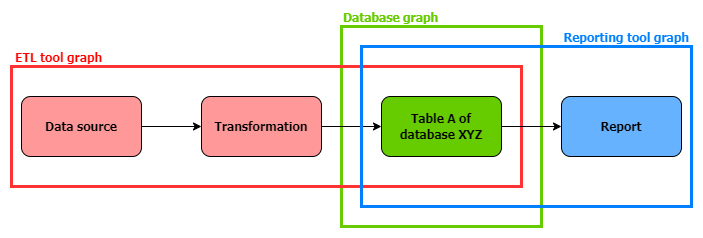
\includegraphics[width=1.0\textwidth]{img/graph_example.png}
\caption{An example of a combined data lineage graph}
\label{figGraphExample}
\end{figure}  

\par
To illustrate this with an example, let us have an ETL tool which contains a pipeline writing data into table A of database XYZ and a reporting tool which visualizes data from this table in a report. The analysis would produce three graphs:
\begin{itemize}
    \item an ETL tool graph which contains data pipeline data flow ending with a write to table A,
    \item a database XYZ graph which represents table A and its columns,
    \item a reporting tool graph that contains data read from table A into a report. 
\end{itemize}
These graphs would be visualized as one unified data lineage, as seen in Figure~\ref{figGraphExample}.

\section{Embedded code}
Various data processing, management and analytic tools have been developed to allow their users to extract important pieces of information from the vast amounts of data they collect. These tools often provide graphical interface for creating data pipelines consisting of commonly used data sources and transformations. Using such tool opens data pipeline management to a wider, less technically proficient audience, so business-oriented employees can be involved more closely in the development. An example of such tool may be AWS Glue platform where users may define their ETL pipeline using graphical interface with multiple data sources, transformations and joins without having to write a single line of code. However, data can be very dynamic and different and it would be difficult to define every possible data transformation that the users might require. In such cases these tools often allow extending the pipeline with embedded code.
\par
Embedded code is a piece of code provided by the user that is safely executed in the context of the tool and can perform (almost) any desired task. It is often a function or a script. Popular examples of tools that support embedded code include already-mentioned AWS Glue, but also Databricks platform, Snowflake data cloud or SQL Server Integration Services (SSIS) etc. Programming languages used in embedded code often include the popular and well-known ones such as Python, Java, Scala or C\#.
\par
Embedded code can be used to perform a data transformation in an ETL pipeline that is not included in the standard toolbox, read data from an unsupported data source or to create a user-defined database function that cannot be written efficiently in SQL.
\par
Data flow analysis of embedded code is a crucial missing link in Manta Flow. It can analyze both data pipeline metadata and standalone Python, Java or C\# applications, but there is no support when such a piece of code is a part of the pipeline. Missing embedded code data lineage causes logical gaps in the holistic data lineage and decreases its usability, because these gaps have to be filled in by hand. Following the recent surge in demand for data science and machine learning solutions where especially Python is the programming language of choice, the number of enterprises that use embedded code in their data environment has also risen significantly. This drives the market demand for data lineage solutions that can cope with it. As there are currently no solutions that can reliably provide such data lineage, extending the current capabilities of Manta Flow to analyze data lineage in application source code with the ability to also analyze embedded code shall provide it a significant competitive advantage.

\section{AWS Glue}

AWS Glue is a serverless data integration service that makes it easier to discover, prepare, move, and integrate data from multiple sources for analytics, machine learning and application development. It performs data processing on Apache Spark engine in a cloud environment. Data pipelines are defined using embedded code, supported programming languages are Python and Scala. They can also be created from the GUI, where the tool generates the corresponding pipeline code. This service is especially convenient for companies that already use other AWS services as it can efficiently use such resources.
\par
AWS Glue has been on top of the list of technologies to be supported by Manta Flow based on customer enquiries. There is currently very limited support for automated AWS Glue data lineage on the market, so offering it provides a competitive advantage. As the pipelines consist of embedded code, analyzing it is the best, although a very difficult way to extract data lineage information. However, Manta Flow can already analyze Python and Bytecode (Scala is compiled into Bytecode) applications. Providing support for embedded code analysis is therefore a direct prerequisite for a successful AWS Glue data lineage solution.

\section{Goals}

The goal of this thesis is to design a data lineage analysis service for embedded code in Manta Flow that will enable integration of data lineage graph from data processing and analytic tools with the data lineage graph derived from the embedded code.
\par
One of the main tasks is to create a solid design of the service that should be easily extendable with support for new tools and their embedded code in the future. Benefits and usefulness of this design will be then demonstrated on a prototype implementation of the service for AWS Glue and the embedded code written in Python.
\par
Other specific tasks include a proof-of-concept implementation of a metadata extractor for AWS Glue and modifications to the existing Python scanner. A very important aspect of the service is high performance, because it will be called many times during a run of the Manta Flow analysis platform, specifically every time the analysis processes a statement that executes a piece of embedded code.

\section{Glossary}

Let us define a few important terms that are often used in this work.
%% TODO
\begin{itemize}
    \item \textit{Data flow} refers to the path and direction of data movement, capturing the sequence of transformations and processing steps that data undergoes throughout its lifecycle.
    \item \textit{Data lineage} is the record of the origin, transformations, and movement of data, providing a clear and traceable path from its source through various processes and systems to its destination.
    \item \textit{Manta Flow} is a state-ot-the-art automated data lineage analysis platform.
    \item We will use the term \textit{data technology} to uniformly reference databases, ETL and reporting tools. This term shall simplify naming all systems, frameworks, platforms and tools that can be used for data processing and management in the work.    
    \item \textit{Manta scanner} is a component of Manta Flow specialized to perform data lineage analysis for one data technology.
    \item \textit{Embedded code} is a piece of code (a script, a class, a package) embedded in a data technology that is executed in a specific runtime environment to perform a specific task.
    \item \textit{Metadata} refers to descriptive and contextual information about data, encompassing details such as data source, format, structure, meaning, and other attributes.
    \item In the context of embedded code analysis, \textit{source technology} is the data technology that uses embedded code, or from a different point of view, a data technology that is the source of embedded code.
    \item \textit{Embedded Code Service} is a service for data lineage analysis of embedded code.
\end{itemize}

\section{Outline}

This thesis is split into several chapters. In introduction we briefly describe the motivation and the goal of the thesis. In the second chapter we describe important aspects of MANTA Flow platform with which the service developed in this thesis is integrated in. Chapter 3 is dedicated to a detailed problem analysis and we formulate our requirements there. Chapter 4 delves into design and implementation of embedded code service and changes that were made to Python scanner. In chapter 5 we take a look at the design and proof-of-concept implementation of AWS Glue scanner, which uses Embedded Code Service for data flow analysis of embedded Python code. In chapter 6 we demonstrate the functionality of implemented features on several examples and discuss the limitations of the implementation. Finally, in conclusion we sum up what we achieved in this work and how we did it.
\chapter{Manta Flow platform}

Before we get into the details of data lineage analysis service for embedded code, let us first introduce and describe Manta Flow platform. It is the platform that the service is integrated with and influences many of the design and implementation decisions. It also provides a couple of solution examples for problems we might face that we will use for inspiration.

%---------------------
% SECTION
%---------------------
\section{Data lineage}

Data lineage refers to the tracking of data from its source to its destination and all the transformations and processes it undergoes along the way. It is the complete end-to-end history of data flow, including its origins, where it has been, and how it has been altered.
\par
The purpose of data lineage is to ensure that data is accurate, trustworthy, and complies with regulatory and compliance requirements. It provides transparency into data transformations, allowing organizations to understand how data has been changed. Data lineage is also used to identify and resolve data quality issues and to support data governance and management initiatives. From an engineering point of view, it can help developers to integrate data from multiple sources more efficiently and ensure that data is accurately transferred and transformed throughout the system. Overall, data lineage plays a crucial role in improving the reliability, efficiency, and effectiveness of data-driven decision-making.
\par
Data lineage can be obtained by hand from teams of analysts that map data environments or, more recently, using one of the automated systems that are being developed. Manual data lineage analysis is time- and labor-intensive, so developing automated solutions can provide more up-to-date results and decrease costs.

%---------------------
% SECTION
%---------------------
\section{Manta Flow overview}

Manta Flow is an automated data lineage platform that scans data environments to build and visualize a graph of all data flows within it. This graph enables its users to get better visibility and control of their data processes.
\par
Manta data lineage graph is a graph consisting of nodes (vertices) and edges between them. A node may represent a data source or a transformation, e.g., a database table column, a report dimension or a union of columns. Edges are directed and represent data flow from one node to the other. Each node is identified by a unique path.
\par
Each data environment consists of a different set of databases, tools and other technologies. In order to build a data lineage graph for the entire environment, Manta Flow uses a wide range of proprietary scanners. Each scanner can analyze data lineage for a single data technology (we will use the term \textit{data technology} to uniformly describe databases, ETL/reporting tools and programming languages supported by Manta Flow platform). These partial graphs are then combined in metadata repository to provide the output for the entire environment.

%---------------------
% SECTION
%---------------------
\section{Scanners}

A scanner provides data lineage for a particular data technology. This process consists of multiple steps and varies for each technology based on its type. The data lineage is created from metadata and scripts, so the execution of a scanner is split into two general scenarios: metadata extraction and dataflow analysis.

\subsection{Metadata extraction}

Metadata extraction usually, as the name suggests, extracts metadata required for the dataflow analysis. Other artifacts could be extracted, too, such as scripts of any kind, configuration etc. The purpose of this scenario is to gather all resources needed for dataflow analysis and store them locally so that the analysis can be executed in \textit{offline} mode, that is, without requiring an active connection to any other system.
\par
Database scanners usually go one step further and create so called \textit{data dictionary} from the extracted metadata. Data dictionary stores schema of extracted database resources in a universal data structure that is able to capture different hierarchical structure.
\par
There are multiple reasons why metadata extraction is a standalone scenario. Here is a list of some that are relevant in the context of this thesis:
\begin{itemize}
    \item The analyzed systems are not directly accessible from \textit{MANTA Flow} server. \textit{MANTA Flow Agent} is a component that can be configured to perform the extraction on a remote device which has network access to these systems and then securely transfer the extracted artifacts back to \textit{MANTA Flow} server. 
    \item When errors occur during extraction, the user can fix them before executing dataflow analysis.
    \item In some cases, the user may want or have to provide additional input, e.g., configuration not provided via any available API, additional mapping information etc.
\end{itemize}

\subsection{Dataflow analysis}

Dataflow analysis discovers data flows in target systems using the extracted inputs. The output of such analysis is a data lineage graph. There are multiple steps in this process and the specifics vary between different technologies. Sometimes it in includes translating structured metadata into nodes and edges, sometimes scripts need to be analyzed.


% Description of query service, how it works, similarities to what we are trying to achieve.
%- it has a common interface
%- usually used when the connection details are not entirely known
%- could also be that nothing is known
%- can deduce
%- only resolves queries for which it constructs nodes
%---------------------
% SECTION
%---------------------
\section{Dataflow Query Service}

Dataflow Query Service is a component that helps with processing of embedded SQL queries. It works by selecting the appropriate embedded language scanner for the provided input, executing dataflow analysis and merging the resulting sub-graph into the graph of the original data technology scanner.
\par
Often, data technologies such as reporting or ETL tools use SQL to define data sources. Such SQL queries are used to query data from a connected database without the need to create a dedicated table or a view. Since Manta Flow contains scanners for most common database systems, they are already able to process these queries. Dataflow Query Service groups these scanners in a unified service that can be used by other data technologies.
\par
One of the main benefits of this service is that it uses metadata extracted by each scanner, therefore it has access to extracted database schemas, which allows it to resolve exact columns for queries such as \texttt{SELECT * FROM TABLE\_A}. It is also useful in situations when details about the target systems are unknown or unresolved, the service has the ability to deduce columns from available information and to choose the appropriate scanner from the provided connection details.

\subsubsection{Overview}
In general, there are three pieces of information needed to analyze an SQL query:
\begin{itemize}
    \item Connection data - connection type, connection string, server hostname (at least connection string or server name is needed).
    \item Default data - default database, default schema, connecting user (as applicable) in case connection data is not available or not recognized.
    \item Query or embedded script text.
\end{itemize}
If the data technology scanner has all of the above information, it constructs a \texttt{Connection} object directly, otherwise it is expected to perform connection mapping by retrieving the required data from manual configuration. Connection and query text are inputs for Dataflow Query Service. Next, dictionary mapping is performed, that is, an appropriate target scanner and a persisted data dictionary is selected based on \texttt{Connection} data. The selected scanner is invoked with query text, data dictionary and defaults, which provides the result in form of a \texttt{DataflowQueryResult}. The data technology then uses this result to connect the resulting lineage to the relevant nodes in the host script and to merge the result into the main graph.

\subsubsection{External connections}
One of the main purposes of \texttt{DataflowQueryResult} is to perform connection to external nodes. The purpose of embedded queries is to provide data for further processing, therefore we would like to connect the nodes of the query objects with other nodes in the lineage, e.g., connect database columns with data fields in a report. These connection points are unknown to the query scanner and the host scanner doesn't understand the query in advance, so the result graph contains extra nodes called \textit{pin} nodes.
\par
Pin nodes represent an input to a node representing query parameter or an output from a query resultset column. After the query is analyzed and its graph is created, the service adds these pin nodes and connects them with appropriate edges to the result nodes. Then, the host scanner might provide a mapping from pin nodes to nodes in the host graph. The service creates new edges from pin nodes to host graph nodes (and vice versa, depending on the direction) based on the provided mapping and then contracts the pin nodes, thus effectively connecting the resultset column node or a parameter node with the host graph node. Should any pin node remain unmatched, it is filtered out in filtering task later in the scenario.

\subsubsection{Architecture}
%%% copied from Confluence, can I somehow quote this?
\begin{figure}[ht]\centering
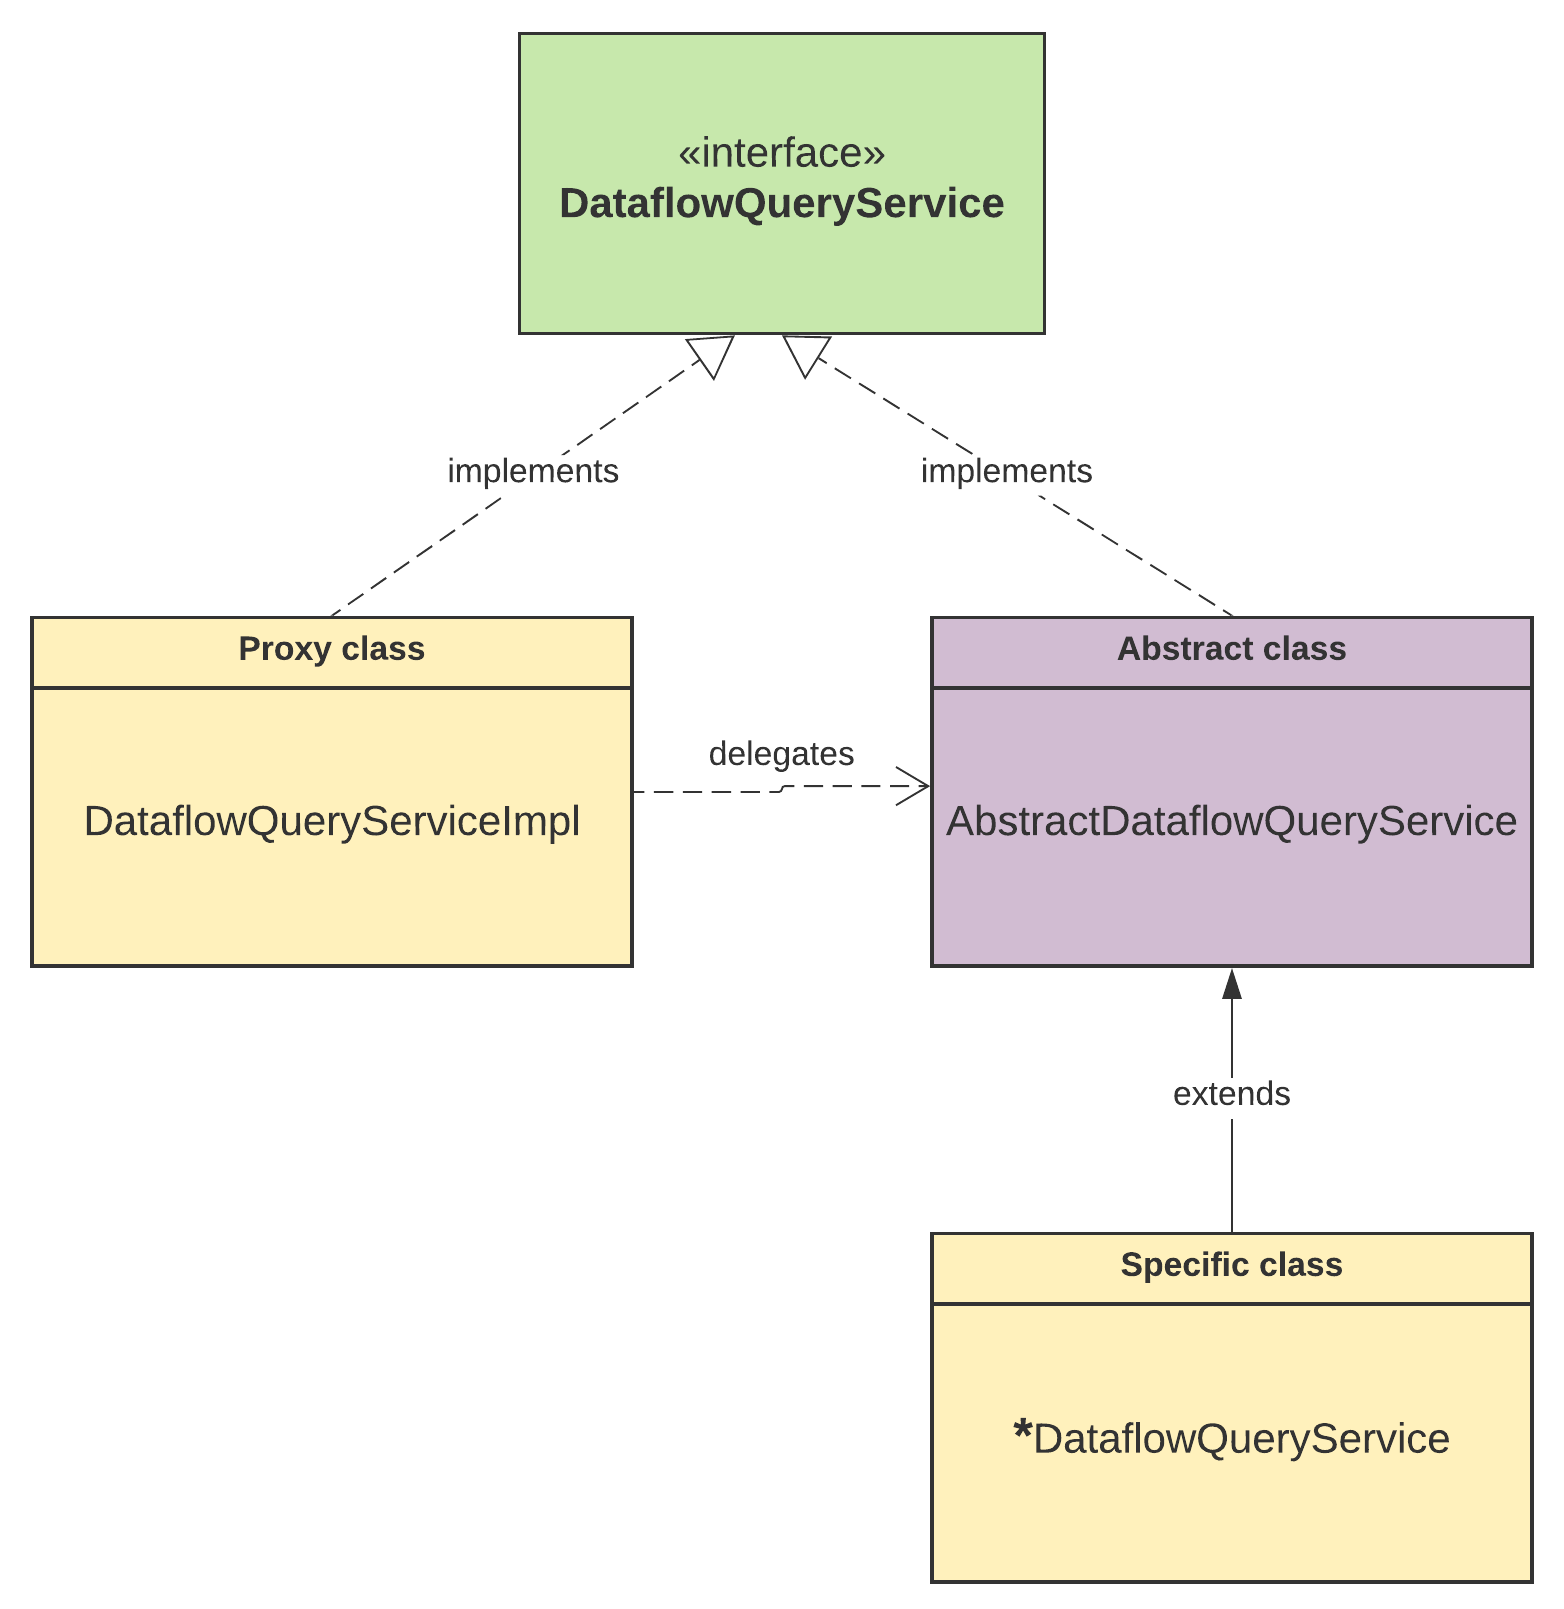
\includegraphics[width=1.0\textwidth]{img/cls.png}
\caption{A simplified class diagram of Dataflow Query Service}
\label{fig01:QS}
\end{figure}  


\texttt{DataflowQueryService} is a common interface that provides methods for client scanners for analyzing SQL queries or creating hierarchical database structures. This interface is implemented by:
\begin{itemize}
    \item Individual database query services that contain logic for providing data flows or hierarchical database structures.
    \item Proxy class called \texttt{DataflowQueryServiceImpl} that wraps all other individual query services. It is a classic implementation of a proxy class that chooses a specific query service based on information provided in the connection from the caller and delegates the operation.    
\end{itemize}

A simplified class diagram is depicted in figure~\ref{fig01:QS}.

% Description of language scanners, their composition, how they work
%- no DDL/dictionaries, only scripts
%- extraction is just a preparation of the input
%- analysis uses worklist algorithm, intermediate dataflow generator, common output
%- differences with database scanners
%- 
%---------------------
% SECTION
%---------------------
\section{Programming Language Scanners}

There are currently three programming language scanners: Bytecode scanner, C\# scanner and Python scanner. Their purpose is to analyze source code and discover data flows there. It proves important to also support this type of data lineage as sometimes the transformation from one data source to the other is implemented in a script or an application. Without this piece of information it is not possible to deliver a complete data lineage.
\par
Programming language scanners are one of the most complex scanners in Manta Flow. The scope of processes that can be expressed in a programming language is much greater and more complex compared to other data technologies. These scanners perform static analysis of the code. Execution of the code is not possible nor wanted and modification of the source code for the purposes of data lineage analysis is usually not possible either because there may be hundreds to thousands of code files included in the analysis which would be very labour intensive. Therefore, static analysis is the only feasible option.
\par
The goal of this static analysis is to find where data is read into the application, track it across all transformations and then find where it is written out. This proved to be a difficult task. There are several approaches for static code analysis, but none of them is aimed at data lineage, so a custom algorithm had to be developed. It uses symbolic analysis and an iterative approach along with multiple optimisations to produce limited results in a limited environment. These limitations are computing power, memory space and time. Manta Flow is expected to run in a common enterprise environment on a machine with a standard multi-core CPU, a reasonable RAM size (e.g. 32GB). Furthermore, the analysis is expected to end in the span of hours up to a few days. Due to that the output focuses on visualizing data reads and writes and flows between them and does not show internal transformations.

\subsection{Dataflow analysis of source code}

Let us describe how this analysis works in more detail. It will help us understand problems and solutions later in this work. All programming language scanners follow a similar workflow, but they implement each step in a little different way due to differences between the languages.

\subsubsection{Source code extraction}

The first step is source code extraction. Before the analysis can begin, all inputs need to be collected and prepared in the format they are expected to be in. The applications usually consist of the application code and of external libraries. When the files are collected, an extraction configuration is generated which captures the structure of the input allows the user to specify which functions or modules should be considered as analysis entry point.
\par
Analysis entry point is the routine that shall be considered as a starting point of a program execution. Usually, it can be the \texttt{main} method in Java or C\# or the module containing \texttt{\_\_main\_\_} block in Python, but in general it can also be any other function, method or module. This defines the starting point of the analysis and from that point function invocations and variable assignments are tracked.
\par
Source code extraction is a standalone step and represents metadata extraction for programming language scanners. All following steps are a part of dataflow analysis.

\subsubsection{Input processing}

In this initial step of dataflow analysis, the extracted inputs are read from file system and pre-processed. In Python, this involves parsing of the source code into an internal representation. There are a couple data structures that need to be created in this step which are used in the following ones.
\par
One of these structures is class hierarchy, which helps with the detection of invocation targets. The other, more important for the algorithm is \textit{call graph}. It captures caller-callee relationship between executables (functions, methods, modules) in the application. A caller is the executable that invokes another executable in its body, a callee is the executable that is being invoked by another executable. Call graph helps to find which other executables need to be analyzed again after the analysis of one, because its result might influence the callers and callees. This will be explained in more detail later.

\subsubsection{Alias analysis}

Aliases are different expressions that might reference the same value. It is important to analyze assignments in the application to resolve these aliases, because a value assigned into one of these expressions has to be propagated into all aliases. Similarly, if a value in an expression is modified, so it is in all of the aliases.

\subsubsection{Symbolic analysis}

This is the core of the analysis. 

\subsubsection{Output transformation}

\subsubsection{Generating data lineage}


\chapter{Requirements and Analysis}

In this chapter we follow up on the Manta Flow platform description and explain the problem of analysing embedded code in this context. We analyze multiple technologies that support embedded code and formulate our requirements for the solution. Then we analyze how to integrate embedded code analysis into scanners.

%%----- SECTION -----%% An extended problem overview, analysis of supported/desired technologies that support embedded code.
\section{Problem overview}
% Why we analyze scripts
Analysis of scripts is an integral part of many scanners supported in Manta Flow. The scripts improve the usability of the data technology as they enable user-defined ways to modify and work with data and even might be the only way to do so. Stored procedures and functions in databases enable data manipulation on top of data storage which can be especially beneficial if the database is accessed from an environment with limited database support. ETL platform scripts allow users to define their own data transformations on top of the well-defined ones. In reporting tools, the scripts provide a handy way to pre-process and define source data for data visualizations.
\par % some scripts are easy to analyze
In most of the cases, these scripts use a more-or-less standardized language native to the platform. Analyzing native scripts has been a standard part of scanners. It provides a lot of value as it covers a great part of data lineage. Since such language is usually an internal part of a particular data technology, its processing algorithm does not need to be shared with other components and it can utilize the internal representation of other entities unique to that data technology. Additionally, these languages do not usually have a strong expressive power, meaning that the breadth of ideas that can be represented in them is limited to the scope of the data technology and is usually  lower than that of standard programming languages.
\par % sometimes a more complex language is used for scripts
Analyzing code written in standard programming languages is considerably more difficult, mainly because the expressive power is that much stronger. It often contain expressions or entire algorithms not relevant for the data lineage, however that only becomes apparent after the analysis. That makes programming language scanners the most complex ones. However, this ability is useful for embedded code scripts. Certain data technologies provide an environment where these scripts can be executed, thus utilizing the potential of strong, well-defined and well-known languages.

\subsection{Analyzing embedded code}
% why we want to analyze embedded code scripts
Adding support for embedded code scripts in a data technology might initially sound like a great idea, but like everything else, it comes with its positives and negatives. We have already mentioned most of the positives. The main negatives from software development point of view are limited debugging, testability and version control support. As already mentioned, embedded code is executed in a custom internal runtime environment of the data technology and its replica for development is not always available. For that reason there is an increased demand for systems that can bridge this gap and verify the embedded code correctness. One of the ways to check it is utilising data lineage analysis to verify that the data flow as expected.
\par % what we need to analyze embedded code
Supporting the analysis of embedded code in Manta Flow is not as simple as running the particular scanner with the code as its input. Since the analysis of programming languages is so complex, we want to use the existing scanners as much as possible. However, original implementations of these scanners were developed to be able to process applications written in the particular programming language. They are designed to run in standalone scenarios and their configuration mostly defines where the application can be found. We need to modify these scanners so they can be reused by other independent data technology scanners in their scenarios in a meaningful way.
\par % how query service does it
A similar problem has been solved by Dataflow Query Service which allows other scanners to process database queries. These database queries need to be processed by a particular database scanner, because different databases use different SQL dialects and also because Query Service results are enriched with the mapping to the actual data sources that has been analyzed by that scanner, if possible. We will inspire by its design because it solves two similar problems: providing a partial lineage graph to be used in another lineage graph and executing the analysis of one scanner in the scope of another.
\par % how we shall do it
Our solution shall provide an embedded code service which can be integrated and used in other scanner scenarios. It shall provide an interface to configure the input and execute the analysis of the provided embedded code and it shall provide an interface to integrate the resulting lineage graph with the lineage graph of another data technology.

%%----- SECTION -----%%
\section{Source technology analysis}

Before we dive further into the analysis, we need to examine which source technologies, whether currently supported by Manta Flow or planned, support embedded code. This overview will give us a better understanding of the range of embedded code use-cases as well as help us in choosing a candidate for a proof-of-concept implementation.

\subsubsection{Hive}
Hive is a distributed data warehouse system that allows users to read, write and manage big volumes of data using SQL. Starting from version 0.13.0, it supports writing user-defined functions in Java which accept parameters and return a value. The function is implemented by a class that extends a Hive UDF base class. These base classes define methods that shall be implemented by the function and will be invoked in specific order on SQL query execution. This class is then supposed to be packaged in a JAR referenced by a URI from which it will be loaded into the environment~\cite{hive}.

\subsubsection{Microsoft SQL Server}
Microsoft SQL Server enables users to implement stored procedures, triggers, user-defined types, user-defined functions (scalar and table valued), and user-defined aggregate functions using any .NET Framework language, including Microsoft Visual Basic .NET and Microsoft Visual C\#. They can be implemented by arbitrary classes and methods as long as they are properly annotated. These annotations facilitate the lookup and binding between SQL Server and embedded code. Compiled code is distributed in DLL and loaded into environment using SQL syntax~\cite{mssql}.

\subsubsection{SQL Server Integration Services (SSIS)}
SSIS is a platform for data integration and transformation solutions. It provides graphical tools for building ETL workflows, but it is also possible to create custom objects programmatically in C\# or Visual Basic. These include tasks, connection managers, log providers, enumerators and data flow components. Implementations of custom objects are expected to extend one of the base classes provided by SSIS, to override required methods and to use proper attributes. These objects are then distributed as a compiled class library. This is a similar approach as that of MSSQL~\cite{ssis}.

\subsubsection{PostgreSQL}
By default, PostgreSQL supports functions written in C, but theoretically users may use any language, as long as it can be made compatible with C, e.g. C++. However, that is often difficult due to different calling conventions, so its safe to assume C language is used. The function definitions are supposed to use macros from \texttt{postgres.h} header file, but otherwise are common C functions. The code is compiled and dynamically loaded into the environment using SQL. There is currently no plan to support analyzing C language, so this data technology is mentioned only for completeness~\cite{postgresql}.

\subsubsection{Snowflake}
Snowflake Data Cloud is a cloud-based data storage and analytics service. It is common to use SQL to interact with data in Snowflake and embedded code is integrated in a similar way in the form of functions and stored procedures. Apart from SQL, these can be written in multiple programming languages - Java, Scala, JavaScript or Python. Each language used has (slightly) different capabilities and requirements. In case of JavaScript, it can be used to execute SQL statements and interact with the result to provide a return value. Java, Scala and Python scripts have to contain a function or a method with the first argument of type \texttt{Session} from Snowflake's Snowpark library. This argument will be populated by Snowflake when the procedure/function is invoked and is used for interaction with Snowflake platform~\cite{snowflake}.

\subsubsection{Databricks}
Databricks is a web-based data platform that combines data warehouses and data lakes with analytics build on Apache Spark and IPython-style notebooks. These notebooks are interactive computational environments. They consist of a sequential combination of cells which may contain rich text, embedded code, data visualization etc. Embedded code cells may be written in Python, Scala, SQL or R and it is possible to combine cells written in different languages in one notebook. During a notebook execution, cells written in the same language are executed in the same environment and may interact with other language environments using shared context of Apache Spark~\cite{databricks}.

\subsubsection{AWS Glue}
AWS Glue is an ETL tool that supports interactive ETL pipeline creation and then generating code for Apache Spark in Python or Scala that executes the pipeline. This code can then be further modified. Compared to other data technologies, AWS Glue is built entirely on embedded code. That means that each ETL job is executed entirely by a single Python/Scala script as opposed to only parts of data operations in other data technologies~\cite{awsglueintro}. 

\subsubsection{Other data technologies}
Besides the data technologies already described, there are others that provide embedded code integration and are supported in Manta Flow. These follow similar principles as some that were already described before, so we will not cover them in detail. However, we list them below for completeness:
\begin{itemize}
    \item Talend supports extending the functionalities of a Talend Job using custom Java commands~\cite{talend}.
    \item Google BigQuery supports defining functions written in JavaScript~\cite{bigquery}.
    \item StreamSets allows creating custom StreamSets processors in Java~\cite{streamsets}.
    \item Informatica supports creating custom components with Java~\cite{informatica}.
    \item Azure Data Factory supports creating Custom activity with own data movement or transformation logic in C\# that can be added to a pipeline~\cite{adf}.
    \item SAS supports running Python statements within a SAS session~\cite{sas}. Additionally, there are multiple Python packages for interacting with SAS from Python.
\end{itemize}

\subsection{Embedded code usage philosophy}
Based on the description of embedded code usages, we can observe a few repeating patterns. These will help us design embedded code service.
\par
We can see that database systems use embedded code in the form of user-defined functions or stored procedures. They can then be invoked as a part of an SQL query or an SQL script. They often return a value and may receive arguments.
\par
Another common use-case is to define a custom transformation or a task in an ETL workflow. The details of this use-case vary more than those in database systems but in general they implement a specific interface which functions are invoked in a pre-determined order by the data technology.
\par
Next observation relies to the programming language being used. Most often we can see Java or Scala, .NET languages (mainly C\# or Visual Basic) and Python. Sometimes also JavaScript is used and there is one case of R and C, but we shall ignore them as there isn't currently a language scanner implemented in Manta Flow for them.
\par
In compiled static-typed languages (Java and C\#), it is common to tag the classes that shall be used as embedded code and require a rigid interface, either by extending a base class or using annotations. The code is distributed in compiled form and loaded dynamically. Interaction with the data technology is facilitated through an object that is provided as a method argument or a property of a base class.
\par
As Python is interpreted and not compiled, it is possible to inject the embedded code into a different code to create a new script. That allows use-cases where some code is executed before embedded code which defines some variables, functions, classes etc. The embedded code may then directly read these identifiers without having to declare them, which is used to provide interface for interacting with data technology. To successfully analyze such approach, it is important to understand and simulate these assignments.

%%----- SECTION -----%% Functional and qualitative requirements
\section{Requirements}

There are a couple of requirements that the embedded code service needs to fulfill. 

\subsection{Functional requirements}
\begin{enumerate}
    \item Provided a code script (string/file, not important implementation detail) and configuration, the service analyzes the script and delivers lineage graph for that script
    \item The service can merge the lineage graph with the lineage graph of parent technology when provided a node to be merged with    
    \item The service can support multiple source technologies - technologies that support usage of user-defined embedded code
\end{enumerate}

\subsection{Qualitative (non-functional) requirements}
\begin{enumerate}
    \item The service should be optimized to handle tens to hundreds of scripts for a specific combination of technology-scanner in one analysis - the limitation should be the speed of the scanner, not speed of the service
    \item Extending supported technologies should be simple - adding a new technology should only include collecting its configuration in the technology scanner and implementing this configuration in embedded code service
    \item Maximizing code reuse - reuse the existing scanners and logic
    \item Minimizing code duplication - no logic should be written on more than one place
\end{enumerate}
\chapter{Design And Implementation Of Embedded Code Service}

Based on the analysis conducted in the previous chapter we now have a clear understanding what Embedded Code Service is, what is its purpose and how it is going to solve outlined problems. In this chapter, we are going to introduce and reason about its design. We are also going to explain what changes need to be done to programming language scanners in order for them to be integrated with Embedded Code Service. At the end of the chapter we will present interesting parts of the implementation based on this design.

\section{Embedded Code Service design}

Firstly, let us summarize the steps that Embedded Code Service has to execute, because it might not be clearly obvious from previous chapters. The goal of the service is to perform data flow analysis of embedded code using one of the already existing scanners to create a data lineage graph of that code which will then be merged with the graph produced by source technology scanner. A programming language scanner works in three steps: extraction of the input, data flow analysis and generating Manta graph. Embedded Code Service needs to perform input orchestration using the provided configuration, then launch all three stages of a scanner and after that help with merging the graphs. The workflow looks as follows (active components are written in parentheses):
\begin{enumerate}
    \item Input orchestration (Embedded Code Service)
    \item Input extraction (scanner's Extractor)
    \item Data flow analysis (scanner's Reader)
    \item Generating lineage graph (Intermediate Dataflow Generator)
    \item Merging graphs (source technology scanner with the help of Embedded Code Service)
\end{enumerate}

\subsection{Multiple programming languages}

The first decision we have to make is whether we want to implement one universal service that can analyze embedded code written in any programming language or whether we want to have specific implementations for each programming language. This decision will greatly influence how the interface of the service is designed.
\par
An initial idea seems to be a universal service, because that is how Dataflow Query Service is implemented. A common service promotes code reuse as multiple parts of the problem will be solved in a similar way regardless of used programming language and data technology, such as merging the graphs of embedded code and source technology. We can also find similarities between the data technologies (e.g., stored procedures written in embedded code in databases) regardless of the programming language used. One service also means that only one component will need to be maintained. The downside of having one service is that its interface needs to be universal, so if one programming language has a different requirement or requires a specific modification, these changes will have to be reflected for other programming languages as well.
\par
One could argue that another benefit of one service is that we have access to the analysis of any embedded code we may find, but that turns out not to be as beneficial as it may sound. In reality, the language of embedded code is always known, so it is easy to use a specific service to analyze it. Having a universal service has been crucial in case of Dataflow Query Service, because it supports recognition of the SQL dialect used in the query, but in case of Embedded Code Service such feature is not needed. When implementing specific services, we can still reach similar code reuse by grouping common logic in base classes, which makes one less argument in favor of a common service. An important advantage that multiple services provide is that they not only allow the interfaces to be tailored to the needs of the programming language scanner, but they also allow different development pace for each service. The fact is that a service for Python is much more preferred by the stakeholders because of its potential and thus a lot more resources are dedicated to working on it.
\par
Comparing the two approaches, we chose specific implementations as a more suitable solution.
The last argument carries great significance due to its profound impact on the development process, so we decided to implement multiple services, each dedicated for one programming language.  
\par
Figure~\ref{fig:ECSbasedesign} shows how a specific service processes embedded code as well as components that is utilizes. The diagram is generic for any programming language.

\begin{figure}[ht]\centering
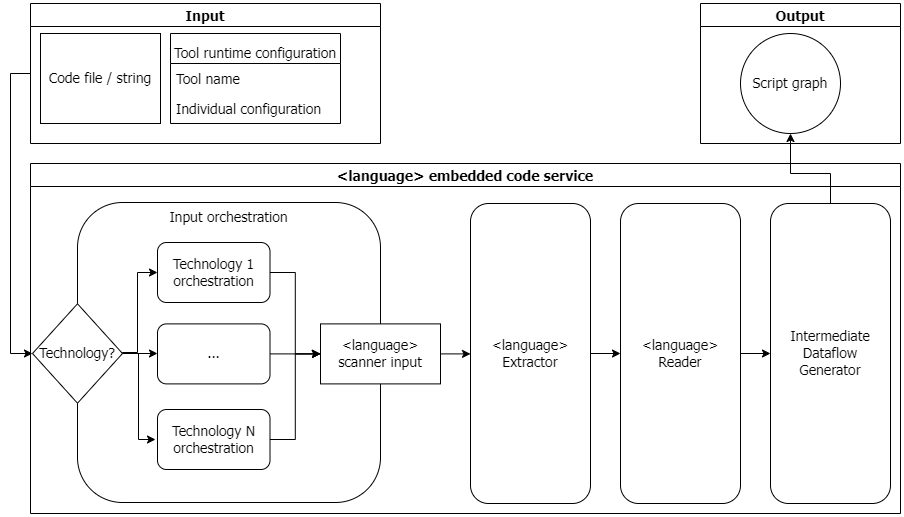
\includegraphics[width=1.0\textwidth]{img/Embedded code service base design.png}
\caption{Diagram of Embedded Code Service workflow}
\label{fig:ECSbasedesign}
\end{figure}   

\subsection{Orchestration}

All contemporary programming languages use some form of import mechanism where the developers can import additional libraries and frameworks. We can see that in embedded code too, often there is a mechanism of adding external libraries to be imported and used by the code. For example in AWS Glue it is possible to define a job argument with a path of Amazon S3 object which contains a custom Python library. When AWS Glue executes a Python job, firstly it checks the S3 location and when it conforms to the required format, it copies the files to the internal working directory next to the job script. When a job is started, Python's import mechanism is able to find these additional libraries and successfully use them in the job script.
\par
Additionally, some technologies (e.g. SAS, Databricks) perform additional orchestration to run the embedded code correctly, such as injecting it in a well-defined class, so this envelope does not have to be written by the user every time, adding the desired imports and only then the embedded code is run on the execution engine used by that technology. This process has to be mimicked by Embedded Code Service before analyzing the code by the scanner to provide an equivalent of the actual code that is executed.
\par
The orchestration process would generally be different for each technology and programming language, but there are some common steps and some repeating patterns. This needs to be reflected in the design of orchestration so the part that needs to be implemented anew when support for new source technology is added is clearly distinguished from common parts. We can use \textit{template method} design pattern, which implements common parts of the process in the base class and lets subclasses redefine certain parts of it. That way we clearly define what can and needs to be implemented.

\subsection{Result}

When the analysis of embedded code is finished, the service shall return a result to source technology scanner. The result is a graph that needs to be merged with another graph and may contain pin nodes that need to be connected. Rather than returning the unfinished graph, we shall return an object that wraps it and provides an interface for connecting pin nodes and merging. The justification is simple, this graph is not always in a valid state so it should be hidden from plain view and unwanted modifications.

\subsubsection{Pin node mapping}
First thing to be done with the result is pin node mapping. This process was described in Section~\ref{sec:pin}. Pin nodes can be found in the graph by enumerating its nodes and filtering those with pin node type. Each pin node can be distinguished from others by its name.
\par
The source technology scanner performing the mapping should receive the information about created pin nodes from an \textit{Insight}. A mapping simply contains a pin node and a node to be mapped to. We might want to connect pin nodes by iterating over them and for each one we create a mapping or we might want to iterate over records in an \textit{Insight}, retrieve the pin node by its name and then create the mapping. Each approach is better in different situations, so the result shall support both operations.
\par
When a mapping is created, it is important to specify whether the pin node is an input node or an output node (relatively to embedded code). The direction decides the orientation of the edge when a pin node is merged to the source technology graph.
\par
During the mapping process, the mapping information is stored and merging is deferred until the end so that the graph remains unchanged throughout the process.

\subsubsection{Merging}
After all pin nodes are mapped, a merge operation can start. This operation can be done only once, because it changes the source technology graph. If it was done multiple times, the graph could be damaged.
\begin{figure}[ht]\centering
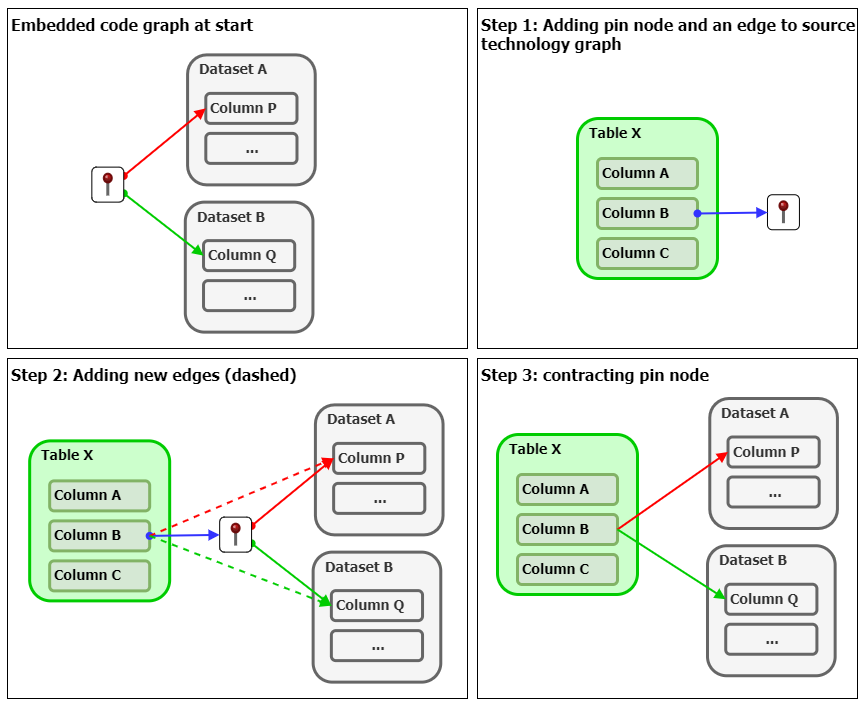
\includegraphics[width=1.0\textwidth]{img/contraction.png}
\caption{The process of merging and contracting a pin node}
\label{fig:contraction}
\end{figure}   
\par
The merging process starts by adding the pin node into the source technology graph along with an edge that connects it to the mapped node. After that, pin node needs to be contracted and removed. That is done by first enumerating its incoming and outgoing edges and adding new edges starting at the starting points of incoming edges and ending at the end points of outgoing edges. After that, pin node and all edges associated with it are removed. A process of contracting a node can be seen in Figure~\ref{fig:contraction}.
\par
When an edge is added to a graph, both its nodes are also added if they were not already present in the graph. After all pin nodes are added to the source technology graph and contracted, all remaining nodes and edges are added and the merging is complete. 

%%----- SECTION -----%% Analysis of Python scanner w.r.t. Embedded Code service
\section{Python scanner changes}

With the design of Embedded Code Service now covered, we need to solve one more issue before we can talk about its implementation. Programming language scanners were not initially designed for running embedded code so we need to look at them and design any required changes in order for them to be used in Embedded Code Service. We will be focusing on changes to Python scanner, because in this work we implemented only Embedded Code Service for Python. Other services were not marked as priorities by the stakeholders in scope of this thesis. However, since all programming language scanners follow a very similar design, the changes done on Python scanner may in the future be (with small tweaks) applied also to remaining scanners.

\subsection{Spring framework}
Before we start with scanner changes, let us have a more detailed look on Manta Flow CLI implementation. It will help us understand some reasons for the changes. Manta Flow CLI is based on the Spring framework. This framework provides a comprehensive set of features and libraries that facilitate the development of robust and scalable Java applications. Among other essential features, we shall look at three of them that we need to understand before following further.
\par
The first important feature is \textit{configuration}. Spring applications typically start with a configuration phase, where developers define the application's beans, dependencies, and other settings. A bean is an object that is managed by Spring. A bean represents a reusable and configurable component of an application. It can be any Java object, ranging from plain Java objects to more complex components. Spring supports two types of configuration, XML-based configuration and Java-based configuration using annotations. Most of the components in Manta Flow CLI use XML-based configuration, however there are some new components in Manta Flow that already use a modern annotation approach.
\par
Second key feature of the Spring framework is its support for \textit{dependency injection}. It allows us to define the dependencies between different components (beans) of the application, and Spring takes care of injecting these dependencies at runtime. This promotes loose coupling and makes the application more modular and easier to maintain.
\par
Lastly, the Spring framework follows the principle of \textit{inversion of control}, which means that the framework is responsible for managing the lifecycle and execution flow of the application. In simpler terms, the application delegates control to the Spring framework, and the framework takes care of executing the appropriate components at the right time.
\begin{figure}[ht]
\begin{lstlisting}[language=Java]
<!-- Define a Spring bean for a simple UserService -->
<bean id="userService" class="com.example.UserService">
   <!-- Inject a dependency using constructor injection -->
   <constructor-arg ref="userRepository" />

   <!-- Set a property value -->
   <property name="maxUsers" value="100" />
</bean>

<!-- Define another Spring bean for UserRepository -->
<bean id="userRepository" class="com.example.UserRepository" />
\end{lstlisting}
\caption{An example of a Spring bean XML configuration and dependency injection}
\label{fig:bean}
\end{figure}
\par
In Figure~\ref{fig:bean} we can see an example of two beans configured in XML: \texttt{userService} and \texttt{userRepository}. The \texttt{userService} bean demonstrates dependency injection by specifying the \texttt{userRepository} bean as a constructor dependency. This means that when the \texttt{userService} bean is created, the Spring container will automatically inject the \texttt{userRepository} bean into it. Additionally, the \texttt{userService} bean showcases property injection by setting the \texttt{maxUsers} property to a value of \texttt{100}. The \texttt{maxUsers} property is assumed to be a property of the \texttt{UserService} class.

%%-subsection-%% 
\subsection{Running the scanner without scenarios}
Each execution of Manta Flow CLI starts a scenario. A scenario consists of a list of steps required to complete a certain task. There are many different scenarios, some are used by scanners. for example various extraction and data flow scenarios, some are used for management of metadata repository in Manta Flow Server. Python scanner consists of two scenarios, \textit{Python Extractor Scenario} and \textit{Python Dataflow Scenario}. Extractor scenario is launched to extract input for Python scanner, dataflow scenario performs data flow analysis and generating lineage graph. Each scenario consists of generic code handling startup and completion of a scenario and specific code performing a dedicated task.
\par
Components of Python scanner, Extractor and Reader, as well as Intermediate Dataflow Generator are currently designed specifically to be started and managed by a Manta Flow scenario. It is desired to modify their design and structure to enable starting the scanners from Embedded Code Service. These modifications should not be big (the scanners are already quite well designed), but they need to be finished before a language scanner can be added to the Embedded Code Service.

\subsection{Python scanner design and Spring configuration}
Python Scanner is designed to analyze user inputs. The source code is stored on the file system by users and its location together with other settings is provided in Spring configuration of the scenario when it is launched. Embedded Code Service also receives the source code, but the configuration is different for each input. As Embedded Code Service is also configured only once at the start of a scenario, this configuration has to be built at runtime, specifically in input orchestration phase. 
\par
Upon analyzing the configuration of Python scanner components we can conclude that they were designed as single-purpose components. They are constructed with all functional elements and input configuration which they need to perform their task. Therefore, the lifecycle of such component ends when it finishes its task and a new component has to be constructed for a new task. This is feasible when Python scanner is executed from a scenario, because each scenario executes each task once. With Embedded Code Service the expected lifecycle of components is different. The service is constructed once but can be used for multiple inputs (e.g., analysis of multiple scripts that are a part of one ETL pipeline).
\par
There are two ways how we can modify current components to support both approaches (service and CLI) efficiently. We can modify the component to become stateless. A stateless component does not hold any internal state and can be used repeatedly. Input configuration and state is managed in an instance of a task context class which is passed to the invocation of any method. The context instance can be constructed at runtime or it can be configured as a bean and injected as a dependency. This approach is best suited for components that have a single entry-point - a single method that is invoked to complete the task, but it is not a condition. In such cases the context object is passed as a method parameter during the execution.
\par
The second approach is to create a factory (using \textit{Factory} design pattern) for a component which will be configured in Spring to store the functional elements for the construction of the component (dependencies). The factory will allow passing the input configuration values as parameters to the factory method which constructs a new component. This approach is suitable for components which hold a complex internal state and it would be costly to refactor them to become stateless component. Also, it is a "cheap" modification, there are no changes required in the existing code, we just need to add the implementation of the factory class and this change needs to be reflected in Spring configuration.

\subsection{Interfaces}
We need to consider one more thing. The components were designed to be used by scenarios in Manta Flow CLI and are customized for that purpose. Often their interface contains a single method \texttt{execute} that performs all the steps required by the scenario. Such interface does not provide the functionality we need in Embedded Code Service, because scenarios often require additional tasks to be done that are not required by the service, e.g. serializing connector output on disk. It would be useful to decouple implementation of the functional component from the scenario interface so the functional component can be used by a scenario and Embedded Code Service but it can have its own interface to perform required tasks.

\subsection{Components}
There are three major components in Python scanner: Extractor, Reader and a shared Intermediate Dataflow Generator. These are the components that need to be modified so that they can be used both by scenarios and Embedded Code Service. Let us have a closer look at each of them and the changes that we made.

\subsubsection{Extractor}
Extractor component was already designed in a convenient way. There is a clear separation between an extractor task implementation used in a scenario (implemented in \texttt{ExtractorTask} class) and the functional component used for the extraction (implemented in \texttt{Extractor} class). The task uses the functional component to perform the extraction and itself implements all necessary interfaces. The design of the \texttt{Extractor} class almost satisfies our conditions, it is designed as a stateless component with the task context defined in a separate class (\texttt{ExtractorConfiguration}), the only difference is that this context is passed to \texttt{Extractor} instances in the constructor and stored. The context instance does not necessarily need to be stored in extractor instance, it was only convenient to do so in the current implementation.
\par
The context contains some file paths pointing to the location of the input or the location of extraction folder, which are read-only and need to be available only during the extraction. This component can be easily refactored to conform to the stateless component approach by removing the context from \texttt{Extractor} instance and instead providing it as a parameter to the \texttt{extract} method, which performs the extraction. When used in a scenario, the context instance is already stored in task instance that contains both context and extractor, so there are no Spring configuration changes needed apart from omitting the context as a dependency of an extractor. When used in the service, the context instance can be easily instantiated using the file paths that the service uses for input orchestration, an extractor will be injected as a dependency of the service.

\subsubsection{Reader}
Python scanner's Reader is a highly state-dependent component. It requires some effort to remove all input-specific information and collect it in a single context instance. Additionally, the current implementation requires refactoring as it does more things than it should. Reader is currently one component that implements both task interface for scenario purposes as well as data flow analysis of Python code done in the scenario.
\par
An increased complexity of the component would make it an ideal candidate for the factory approach, but after a deeper analysis we concluded that using this approach would only postpone important changes. The component does two tasks that are demanded by the scenario, but only the analysis needs to be done for embedded code, the other task is serialization of intermediate results for logging and debugging purposes which is not required by Embedded Code Service. Therefore also this interface needs to be fragmented at which point it is worth the time to make a complex refactoring and convert the component to a stateless one. To satisfy all required conditions we need to:
\begin{enumerate}
    \item Decouple task interface from the Reader implementation
    \item Identify stateless functional sub-components of Reader that can be reused 
    \item Identify state information that needs to be stored in a task context instance of Reader
\end{enumerate}
\par
We have split the original \texttt{PythonReader} class implementation into three new classes: \texttt{PythonReader}, \texttt{EntryPointAnalyzer} and \texttt{AnalyzerConfiguration}. \texttt{EntryPointAnalyzer} is a stateless functional component that performs data flow analysis of a single entry point. In Python data flow analysis, an entry point is a module or a function where data flow analysis begins. When analyzing embedded code, there is always only one well-defined entry point, in application analysis there may in general be multiple entry points. This component will be a reusable dependency of both Reader and Embedded Code Service used for analyzing entrypoints. To analyze an entry point, it requires an entry point specification and analyzer configuration.
\par
\texttt{AnalyzerConfiguration} is a component holding context which is used by \texttt{EntryPointAnalyzer}. It is like a small toolbox that the analyzer uses during the analysis. A new configuration has to be provided for each input, not for each entry point. The reason is that there are certain components that can be shared across multiple entry points of one input to improve performance, such as service for parsing Python code as the code files are common for all entry points, thus they only need to be parsed once. A new analyzer configuration has to be created for each input of Embedded Code Service, only one is required in a scenario.
\par
Lastly, \texttt{PythonReader} class has been modified to work as an implementation of Reader component used by data flow scenario. Internally it uses an entry point analyzer and its own analyzer configuration to analyze all entry points one after the other defined in the input. 
\par
With these modifications, the Spring configuration had to be split in two parts so that the dependencies can be correctly resolved. First one is a general configuration that provides an \texttt{EntryPointAnalyzer} bean. The other is a scenario-specific configuration that creates the \texttt{AnalyzerConfiguration} bean and injects it to a \texttt{PythonReader} bean along with an imported analyzer bean.

\subsubsection{Intermediate Dataflow Generator}
Intermediate Dataflow Generator is a shared component that can be configured and used by any of the programming language scanners. We had to make sure that it keeps this property after all the changes. Generator has been recently refactored and the new implementation already follows many of the principles of a stateless component. However, converting it to a stateless component was not the main focus of the mentioned refactoring so we still need to do some additional changes. There is a similar problem as in Reader that the Generator class implements both a task for the scenario and generating data lineage graph. By splitting it into two classes, one for the purposes of the scenario and the other for generating data lineage graph, we can easily create a stateless component which can also be used by Embedded Code Service.
\par
After the refactoring, a new \texttt{DataflowGenerator} class is the stateless component of Intermediate Dataflow Generator. \texttt{ProgramConfiguration} is a new class introduced to hold context information about a new input. Lastly, a refactored \texttt{TransformationTask} class is now just the implementation of the scenario task, previously it represented all of these new components.
\par
While these changes of Intermediate Dataflow Generator required little code modifications, it resulted in big changes in its Spring configuration. The Spring configuration of Intermediate Dataflow Generator is layered into multiple levels to introduce modularity. This modularity is important as there are currently 3 language scanners that utilize the generator and each of them is slightly different. Moreover, with the introduction of Embedded Code Service, there is another use-case with different needs. The new design reduces the amount of beans that it depends on to a bare minimum and avoids the need to define beans that are unused.
\par
Currently, there are two possible configuration compositions. One is for scanners that are not supported in Embedded Code Service and the other for those that are. For that purpose the configuration of common beans is split in two. Base configuration sets up the core stateless \texttt{DataflowGenerator} component that can also be used by Embedded Code Service. The other configuration sets up also context beans and scenario task bean that is required for CLI integration. These configurations are then included in scanner-specific configuration that provides scanner-specific beans.
\par
When Embedded Code Service is not implemented for the programming language, the situation is simple as Generator is only used from a scenario, so only the scanner-specific beans need to be provided. In Figure~\ref{fig:generatorNoECS} we can see that the configurations are \textit{layered} one on top of another. Each \textit{layer} creates new beans using the beans provided by the previous one, as seen in \textit{composition} diagram. In \textit{dependendencies} diagram we can see what beans the configuration provides to the others and which it depends on. An arrow shows that a bean is available in the configuration at its beginning and is required by the configuration at its end.
\begin{figure}[ht]\centering
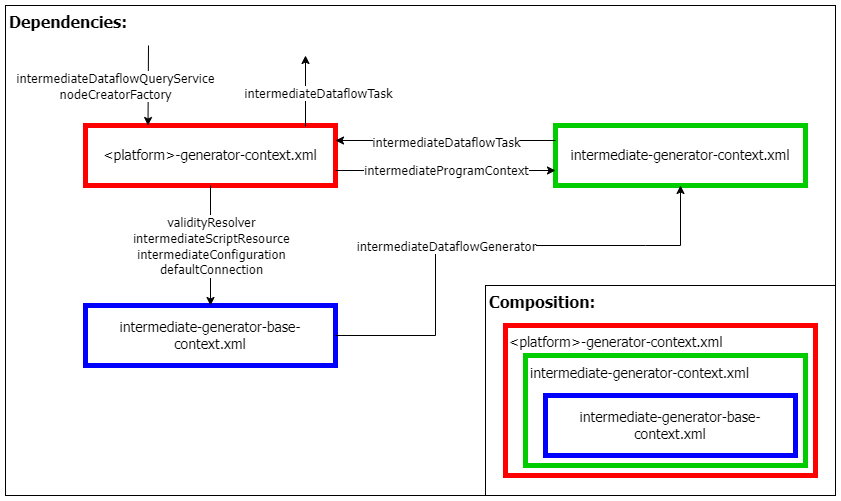
\includegraphics[width=1.0\textwidth]{img/generator_no_ECS.png}
\caption{Composition and dependencies of Generator configurationswhen Emebedded Code Service is not supported for that programming language scanner}
\label{fig:generatorNoECS}
\end{figure} 

\subsubsection{Composition with Embedded Code Service}
When Embedded Code Service is involved, there needs to be one configuration that satisfies the scenario use-case and there can be another one that satisfies Embedded Code Service needs. Embedded Code Service does not need the scenario beans, in fact, they add useless functionality for such use-case, so its best to avoid it. Moreover, in this use-case there could be multiple program configurations passed to Intermediate Dataflow Generator during its lifecycle which cannot be defined statically in Spring. To satisfy these needs the scanner-specific configuration is split in two parts. First part is configuration of common beans for both use-cases and then there are two specializations that utilize common beans - scenario (CLI) and service specialization.
\par
Figure~\ref{fig:generatorECS} shows a different, more complex composition of individual configurations. Similarly to the previous case, \textit{dependencies} diagram shows what beans the configuration provides to the others and which it depends on.
\begin{figure}[ht]\centering
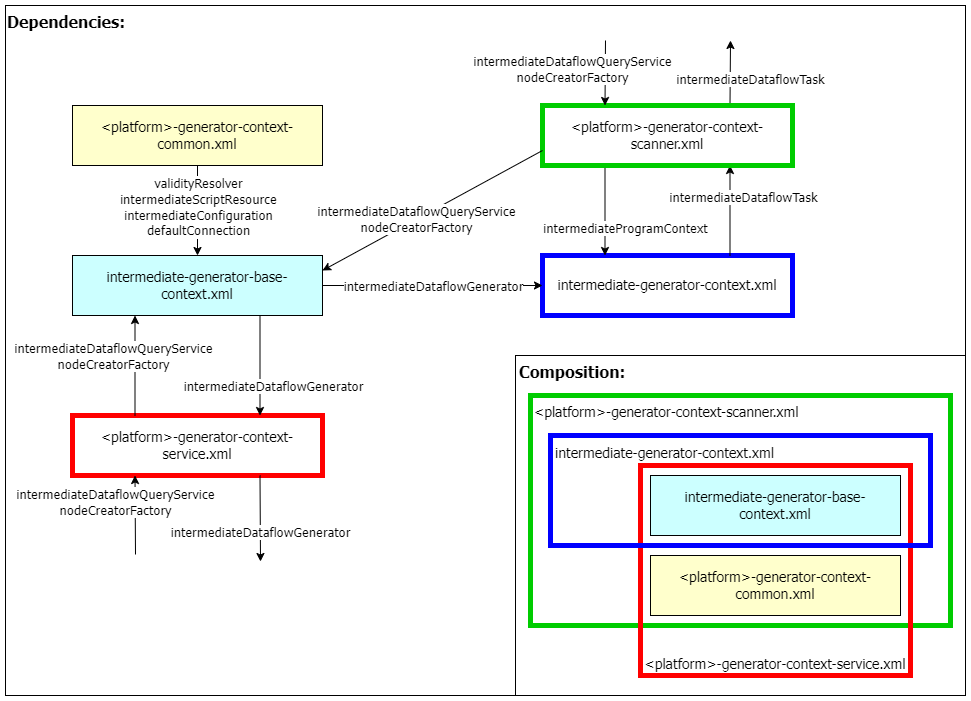
\includegraphics[width=1.0\textwidth]{img/generator_ECS.png}
\caption{Composition and dependencies of Generator configurations when Embedded Code Service is supported for that programming language scanner}
\label{fig:generatorECS}
\end{figure}

\subsection{Insight and Outsight}
There is one more change that we would like to present. Even though it was not implemented as a part of this work, it is a part of the required scanner changes to facilitate its usage in Embedded Code Service, so it makes sense to mention it. We are talking about \textit {Insight and Outsight} mechanism that is used for pin node mapping, but can in general be used to send metadata for embedded code analysis from source technology scanner as well as to receive additional metadata generated during such analysis to be used by the source technology scanner.

\subsubsection{Insighter}
\textit{Python Insighter} is a way how to provide insight into Python code analysis for external consumers. The main idea is to collect events that are important for the external consumer, but which otherwise should not affect Python analysis. Each external consumer has to implement its own \textit{Insighter} specialization together with collaborative propagation modes needed for the specific data technology. Collaborative propagation modes do not propagate data flows, but instead record events into the specialized \textit{Insighter}. After the analysis is complete, an immutable \textit{Insight} object is created which contains the recorded events and can be used by an external consumer.
\par
We can categorize events into data events and lineage events. They need to be handled differently based on their category. Data events are events where we need to know an exact data value regardless of its origin, e.g. SQL query, database connection string etc. For the consumer, the concrete value is the important part, which is recorded in the \textit{Insight} object. Lineage events are the opposite to data events. The exact value is not important in this case, but rather we track these events to create data lineage graph, e.g. reading from a file or a database. The difference from data event is that on top of recording the event into the \textit{Insighter}, a pin node is created and registered as well. After the analysis ends, the external technology can utilize the recorded information to map pin nodes.

\subsubsection{Outsight}

To propagate external information for Python analysis, we can use the Insighter idea and apply it in a reversed manner. \textit{Outsight} object represents events propagated into the analysis. It can use collaborative propagation modes to convert external events and values into Python data flows. \textit{Outsight} can be used for example to create input pins or set values of variables configured in an outside environment.

\subsubsection{Workflow}

\begin{figure}[ht]\centering
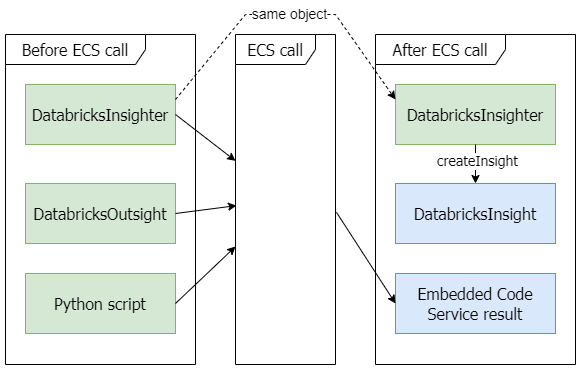
\includegraphics[width=1.0\textwidth]{img/insighter.png}
\caption{Workflow of using Insighter along with Embedded Code Service in Databricks scanner}
\label{fig:insighter}
\end{figure}

Let us present the workflow of this mechanism as it is used in the scanner for Databricks. This scanner was developed along with Embedded Code Service and uses it for analyzing Python code cells in Databricks notebooks.
\par
Figure~\ref{fig:insighter} shows how Insighter objects are created and used in Databricks scanner when calling Embedded Code Service. Before embedded code is analyzed, Databricks scanner prepares analyzed script and stores any contextual information needed for its analysis in an Outsight object. It also creates a new Insighter. These arguments are passed into an Embedded Code Service call, Insighter and Outsight are a part of configuration. After the call is complete, Embedded Code Service produces a result object. At this point, Databricks scanner can get an Insight object from the Insighter and use it to merge the result into its data lineage graph.

\section{Python Embedded Code Service implementation}

Changes implemented in Python scanner were a direct prerequisite to enable an implementation of Python Embedded Code Service. Without them the service would not be able to run code analysis. Having explained these changes, we can now discuss interesting details of the implementation of this service.
\par
Python Embedded Code Service is implemented as a standalone service intended to analyze Python embedded code. It implements two important steps - orchestrating the input in a digestible format for Python scanner and merging the resulting Python graph into the graph of the source technology. The rest of the process is delegated to Python scanner.

\subsection{Interface}

The interface of Python Embedded Code Service contains only one method: \texttt{getDataflow}. This method consumes name of the script, the content of the script, script parent node and configuration. It returns \texttt{PythonEmbeddedCodeResult} object which contains a data lineage graph of the analyzed script.
\begin{itemize}
    \item Name of the script is used for identifying script nodes in the graph and also for debugging purposes.
    \item Contents of the script can be provided in a file or in a string. A typical workflow of a source technology would prepare such scripts during its extraction and store them in files. These files can be directly used as the input or, if they are not Python source files, the code can be provided in a string.
    \item Parent script node is the node that represents the script in the graph of source technology. All nodes in the embedded code graph will use this node as their parent for proper identification.
    \item The configuration stores the runtime/environment configuration for the current script. One script could be run in different environments, with different parameters or with additional user-provided libraries. Configuration that changes between scripts (is not same for each script of given technology) can be passed in this parameter. The specialized implementation of configuration only needs to implement a method that tells its kind (for safe type casting), the rest of it can be freely implemented for source technology needs.   
\end{itemize}

\subsection{Result}
The return value of Python Embedded Code Service is implemented in \texttt{PythonEmbeddedCodeResult} class. It is implemented in a similar fashion as the return value of Dataflow Query Service. It does not provide the result graph directly but instead provides an interface for connecting the two graphs. This interface contains methods for the lookup of pin nodes in the result and creating pin node mappings. After all the mappings are created, we can call \texttt{mergeTo} method which merges result graph with source technology graph provided as an argument. After this operation the result is considered to be consumed and cannot be used again.

\subsection{Orchestration}
The orchestration component prepares the input for data flow analysis. This is done in three steps: input orchestration, extraction and processing of extracted input.
\par
The component is implemented using \textit{template method} pattern. This pattern allows creating a template for a method where some steps of can be reimplemented and the rest is common. The pattern was chosen to encapsulate differences in input preparation for different source technologies into individual classes. The method works as follows:
\begin{enumerate}
    \item Common: a temporary input directory is created. In this directory there is space for preparation of the input for the extractor as well as space for the extractor output.
    \item Specific: input preparation. A specific orchestrator for data technology prepares the input based on the configuration.
    \item Common: the service creates a new Extractor context and runs extraction using Python Extractor and the context. The extracted output is placed in the temporary directory.
    \item Common: the service processes the extracted input by locating the entry point and creating a new analyzer configuration.
\end{enumerate}
\par
Entry point location and analyzer configuration are the outputs of orchestration and are used by entry point analyzer to analyze data flows.

\subsection{Testing}

Python Embedded Code service is covered by both unit and integration tests.
\par
Unit tests verify functionality of individual classes, e.g. orchestrators storing files in correct locations or that pin node mapping is done correctly.
\par
Integration tests verify that all components of Python Embedded Code Service are integrated and cooperate correctly. These tests run the service on different inputs and check that the lineage graph looks as expected after the analysis and merging.
\par
Code coverage by tests reaches 64\% according to SonarQube, a code quality tool used in Manta. This number can be considered lower than standard, but we need to look why that is. The bulk of the uncovered lines are bodies of \texttt{equals} or \texttt{toString} methods along with logging messages which do not require code coverage. In combination with a low amount of code lines in Python Embedded Code Service it results in a lower coverage percentage, but the service can be considered sufficiently covered by tests.
\chapter{AWS Glue Scanner}

The previous chapters were devoted to Embedded Code Service. In this chapter, we will cover the details of the development of AWS Glue scanner prototype. AWS Glue is one of the data technologies that uses embedded code, so we will see how Embedded Code Service service can be used in data lineage analysis. To begin, we will describe AWS Glue and discuss it in terms of data lineage analysis. Next, we discuss and justify the design of a minimum viable product (MVP) of AWS Glue  scanner. Finally, we will look at its implementation. 

%%----- SECTION -----%%
\section{Motivation}

We have already briefly introduced AWS Glue in Section~\ref{sec:sourceTechnologyAnalysis}. Before we dive deeper into its analysis, we shall explain why we picked AWS Glue to demonstrate Embedded Code Service capabilities.
\par
The decision to implement Embedded Code Service in Manta Flow was motivated by the demand to analyze embedded code in several data technologies. Out of the existing programming language scanners in Manta Flow, Python scanner seemed to be the most prospective one to offer attractive value to customers for two reasons: it is widely used and the scanner yielded promising data lineage results.
\par
At this point, there were two options for selecting the data technology for MVP implementation. We could either choose an already supported one that uses embedded Python code to extend its capabilities or create a new scanner for an unsupported data technology. For the first option, could choose SAS, but there was no demand for such feature as Python support has only recently been added into it. For the second option, there have long been plans for AWS Glue and Databricks scanners based on customer demand, both of which use Python extensively. Out of these two, AWS Glue uses Python in a more straight-forward way as AWS Glue jobs are in fact complete Python scripts, which was close to what Python scanner could already analyze with limited results.

\section{AWS Glue analysis}

Before we can start designing the scanner, we need to analyze how AWS Glue works, how it processes data, what metadata it stores and how we can read it etc. 

\subsection{Overview}

AWS Glue is a cloud-based data integration service for discovering, cataloging and transforming data. It is a \textit{serverless} service, which means that there is no dedicated server which requires setup or maintenance. Each execution is managed by AWS Glue which allocates computing capacity on one of the machines in the data center, executes the task and then frees the resources for any other task. The customer does not need to perform any maintenance, they only pay for used computing capacity and instead may focus on developing their data processes.
\par
AWS Glue provides its users several key features:
\begin{enumerate}
    \item \textbf{Data Catalog}: AWS Glue includes a centralized metadata repository, known as the Data Catalog. It stores metadata information about the data sources, tables, and schemas, making it easier to discover and understand the available data.
    \item \textbf{ETL jobs}: AWS Glue allows users to define and run ETL jobs using a visual interface or by writing custom code. ETL jobs enable data transformations such as filtering, aggregating, and joining data from different sources.
    \item \textbf{Data crawling}: AWS Glue can automatically discover and catalog data from various sources, including databases, data lakes, and file systems. It uses crawlers to scan the data sources, infer schemas, and create tables in the Data Catalog.
    \item \textbf{Data preparation}: AWS Glue provides capabilities for cleaning and preparing data before it is used for analysis. It offers built-in transformations and mappings to standardize and transform data, as well as options for creating custom transformations using Python or Scala.
    \item \textbf{Integration with other AWS services}: AWS Glue integrates with other AWS services, such as Amazon S3, Amazon Redshift, and Amazon Athena, allowing users to seamlessly move and transform data between these AWS services.
\end{enumerate}
\par
These features are split into two modules: \textit{Data Integration and ETL} and \textit{Data Catalog}.

\subsubsection{Data Integration and ETL}
The core of data integration in AWS Glue are ETL jobs executed on Apache Spark. Apache Spark is an open-source, distributed computing system that enables fast and flexible processing and analysis of large-scale data sets. It utilizes in-memory computing to accelerate iterative computations, making it ideal for big data workloads. With its distributed architecture, Spark can seamlessly distribute data and processing tasks across a cluster of computers, enabling parallel execution and efficient resource utilization. Spark provides a rich set of libraries and APIs for various data processing tasks available in several programming languages including Python and Scala.
\par
AWS Glue ETL jobs always contain a job script written in Python or Scala which is executed on Spark cluster configured in AWS Glue. Besides writing your own code, AWS Glue provides a tool with graphical user interface for creating ETL jobs. They can be created using transformations and data sources from the tool's toolbox. The tool auto-generates Python script based on the visualization. This script can then be authored, but after that is can no longer be modified in the graphical tool.
We can see an example of an ETL job created in this tool in Figure~\ref{fig:visualJob}. This job reads a table from Data Catalog, renames some of the columns and filters out others and stores the result in a JSON file on Amazon S3, creating a Catalog table for it. Figure~\ref{fig:visualScript} shows the code generated by the tool and illustrates how ETL jobs written in Python look like.
\par
A part of data integration is also scheduler for running jobs periodically or on custom triggers. The jobs can also be organized in a \textit{Workflow}, which is a different form of scheduling where multiple jobs can be executed in the order defined in the Workflow including various conditions and triggers.

\begin{figure}[ht]\centering
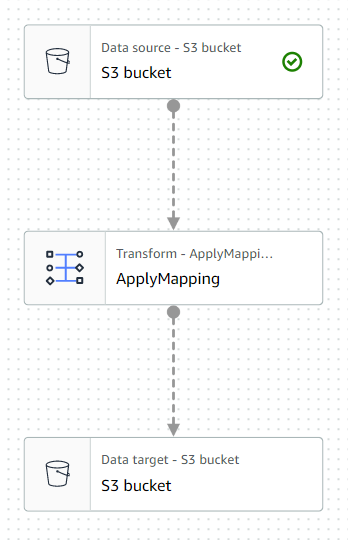
\includegraphics[height=0.6\textwidth]{img/job_example_visualization.png}
\caption{An example of an ETL job created in the graphical tool of AWS Glue}
\label{fig:visualJob}
\end{figure}

\begin{lstlisting}[language=Python,caption=Code script generated in AWS Glue for the ETL job created in a visual tool shown in Figure~\ref{fig:visualJob},label=fig:visualScript]
import sys
from awsglue.transforms import *
from awsglue.utils import getResolvedOptions
from pyspark.context import SparkContext
from awsglue.context import GlueContext
from awsglue.job import Job

args = getResolvedOptions(sys.argv, ["JOB_NAME"])
sc = SparkContext()
glueContext = GlueContext(sc)
spark = glueContext.spark_session
job = Job(glueContext)
job.init(args["JOB_NAME"], args)

# Script generated for node S3 bucket
S3bucket_node1 = glueContext.create_dynamic_frame.from_catalog(
    database="example_db", table_name="wdicountry_csv", transformation_ctx="S3bucket_node1"
)

# Script generated for node ApplyMapping
ApplyMapping_node2 = ApplyMapping.apply(
    frame=S3bucket_node1,
    mappings=[
        ("country code", "string", "country code", "string"),
        ("short name", "string", "short name", "string"),
        ("table name", "string", "table name", "string"),
        ("long name", "string", "full name", "string"),
        ("2-alpha code", "string", "2-alpha code", "string"),
        ("currency unit", "string", "currency", "string"),
    ],
    transformation_ctx="ApplyMapping_node2",
)

# Script generated for node S3 bucket
S3bucket_node3 = glueContext.getSink(
    path="s3://examplebucket/wdi_country_filtered/",
    connection_type="s3",
    updateBehavior="UPDATE_IN_DATABASE",
    partitionKeys=[],
    enableUpdateCatalog=True,
    transformation_ctx="S3bucket_node3",
)
S3bucket_node3.setCatalogInfo(
    catalogDatabase="example_db", catalogTableName="wdi_country_filtered"
)
S3bucket_node3.setFormat("json")
S3bucket_node3.writeFrame(ApplyMapping_node2)
job.commit()
\end{lstlisting}

\subsubsection{Data Catalog}
Data catalog is a centralized metadata repository than can not only be used in AWS Glue, but also in other AWS services. The purpose of Data Catalog is to organize many different data sources in a comprehensible catalog which improves data discovery and utilization. In big data environments and especially in cloud there are many different data sources with different access rules, structure, format and schema. Data Catalog extracts this metadata from each of the data sources and stores it in an abstract structure consisting of databases, tables and columns. A user of Data Catalog then has the ability to uniformly browse and examine them regardless of the actual data source type. Data Catalog can also be used in ETL jobs to simplify reading or writing data, because each resource from Data Catalog is treated the same way in code.
\par
New resources can be added to Data Catalog manually, but its core feature is automated data \textit{crawling} and \textit{classification}. Crawling is the process of exploring resources stored in a data source and classification is the process of inferring data schema in each of the resources. A common use case is to periodically crawl a bucket in Amazon S3 to discover new files and add their schema to Data Catalog using a classifier. AWS Glue provides crawlers and classifiers for most of the common data sources and formats, but it is also possible to write custom ones or browse AWS marketplace.

\subsection{Data lineage in AWS Glue}
To correctly analyze data lineage in AWS Glue, we must first explore which parts of it participate in data pipelines and may contain data flows. It is easy to see that we must analyze ETL jobs as they contain ETL pipeline code and Data Catalog which contains metadata of data sources that could be used in ETL jobs. It turns out that this is all that we need for complete data lineage.
\par
While Workflows seem like they could participate in data lineage, in fact they are used just for job scheduling. If jobs in a Workflow depend on each other, we can see it from just analyzing the jobs, because they would use common data sources through which they would be connected in data lineage graph. The order in which they are executed does not play any role in data lineage analysis.
\par
Crawlers and classifiers in Data Catalog may also contain executable code, but this code just enumerates resources present in a data source in case of crawlers and infers data schema of these resources in case of classifiers. There are no data flows in data lineage context, no values are moving from one place to another. They do not need to be analyzed, but we can read the results of their work in Data Catalog.

\subsection{AWS Glue API}
Now that we know which entities of AWS Glue we want to analyze, let us have a look at how we can get access to their metadata which we will need for the analysis. AWS Glue is usually managed from AWS console, which is a web application for controlling any AWS service. For programmatic access AWS services also provide rich API. It is common that any action that can be made in AWS console has an equivalent support in API. AWS is one of the biggest providers of cloud services worldwide so it should not be a surprise that there are many available SDKs (software development kits) for popular programming languages that support using APIs of AWS services. These SDKs are released under Apache License so we are free to use and distribute them and we can even modify them should we need to do so.
\par
As Manta Flow scanners are developed in Java, naturally the first option was to explore SDK for Java. AWS Java SDK is currently in version \textit{2.x}. This SDK contains multiple packages for each AWS service including AWS Glue. There is a comprehensible API reference and documentation for this SDK available on AWS Glue website as well as a library of examples available on GitHub which explains common usage of the SDK. Overall, this SDK is suitable to fulfill our requirements and needs. We can use it to extract all necessary metadata from AWS Glue.

\subsubsection{Security and access permissions}
It is important to understand how security and access permissions work in AWS Glue. The scanner has to read metadata of sensitive resources. It is important that it can do so in a secure way, otherwise Manta Flow users will not be willing to provide required permissions. Additionally, we need to be able to explain the users exactly what credentials and permissions we need to set up a connection for AWS Glue.
\par
AWS provides a web service called AWS IAM (AWS Identity and Access Management) that helps managing access to AWS resources securely. IAM allows controlling and managing user identities, permissions, and access to various AWS services and resources within an organization.
\par
With IAM, one can create and manage IAM users, groups, and roles. IAM users are specific identities that represent individuals or applications that interact with AWS services. IAM groups are collections of users with similar permissions, making it easier to manage permissions for multiple users. IAM roles are used to delegate access permissions to entities outside of organisation's AWS account, such as other AWS accounts or services.
\par
IAM enables setting fine-grained permissions for users, allowing to control which actions they can perform and which resources they can access. It follows the principle of least privilege, which means users are granted only the permissions necessary to perform their tasks, enhancing the security of organisation's AWS infrastructure.
\par
Overall, AWS IAM allows organisations to create tailored permissions for accessing only those AWS Glue resources that they want to analyze in Manta Flow which builds their trust in this solution.
\par
It is necessary to generate programmatic user credentials to be able to access AWS services from the SDK. These credentials consist of an access key ID and a secret key. This has to be done by organisation's AWS administrator.

\subsection{ETL job metadata}
Let us have a look at what ETL job metadata is available in SDK so we can determine what we can use for data flow analysis. Below is a comprehensive list of interesting properties of job metadata that are relevant for data lineage analysis. We decided to omit some non-relevant ones as the complete list is too extensive~\cite{gluejobs}.
\begin{itemize}
    \item \textbf{Name} – string that identifies a job.
    \item \textbf{Command} – A \texttt{JobCommand} object containing detail about executed command.
    \begin{itemize}
        \item \textbf{Name} – string identifying command type. There are 3 command types: \texttt{glueetl} is a standard Spark job, \texttt{pythonshell} is a job using standard Python shell (without Spark), \texttt{gluestreaming} is a streaming Spark job that runs continuously consuming data from streaming sources such as Apache Kafka. 
        \item \textbf{ScriptLocation} – string specifying the Amazon S3 path to a script that runs a job.
        \item \textbf{PythonVersion} – string specifying the Python version being used to run a Python shell job. Python scanner only supports Python version 3.    
    \end{itemize}
    \item \textbf{DefaultArguments} – A map array of key-value pairs where each key and value are strings. Contains the default arguments for every run of this job.
    \item \textbf{NonOverridableArguments} – A map array of key-value pairs. Contains arguments that cannot be overriden.
    \item \textbf{Connections} – A list of connections used for this job.
    \item \textbf{GlueVersion} – string specifying AWS Glue version which determines the versions of Apache Spark and Python available in a job.
\end{itemize}
\par
Each ETL job has a unique name that can be used for its identification. A job executes a specific command that consists of the environment, job script and arguments.
\par
There are 3 different command types but none of them influences how Python scanner analyzes the script. Presence or absence of Spark environment can be inferred from the script. When Spark functions are used, we can expect that Spark is available, otherwise the script would fail.
\par
Each script is stored in Amazon S3 which means that we need to download it from there in order to analyze it. Users are required to provide sufficient permissions for this action when configuring credentials.
\par
Each ETL job can be parameterized by arguments which consist of default, non-overridable and standard arguments defined on a job run. A complete set of arguments used to run a job can only be found by examining the history of job runs. Arguments can be accessed in the script by calling a dedicated function. Some of the arguments can be used to set up the script environment for the jobs and job runs. There are 4 of them which we need to be aware of:
\begin{enumerate}
    \item \texttt{-{}-additional-python-modules} specifies a list representing a set of Python packages to be installed. It is possible to install packages from PyPI (Python Package Index) or provided in a custom distribution. A custom distribution entry is the Amazon S3 path to the distribution. These packages are available to be used in the job script.
    \item \texttt{-{}-extra-files} contains a list of Amazon S3 paths to additional files, such as configuration files that AWS Glue copies to the working directory of the script before running it. These files can be referenced in the script using a relative path.
    \item \texttt{-{}-extra-py-files} contains a list of Amazon S3 paths to additional Python modules that AWS Glue adds to the Python path before running the script. These modules are available to be used in the job script.
    \item \texttt{-{}-scriptLocation} contains an Amazon S3 location where the ETL script is located. This parameter overrides a script location set in job metadata.
\end{enumerate}
Lastly, jobs can use certain \textit{Connections} defined in Data Catalog. Only the Connections specified in this job parameter can be used. We will explain what they are in the following section.

\subsection{Data Catalog metadata}
We shall also look at available metadata for Data Catalog. There are three types of entities that are useful for data lineage analysis: databases, tables and connections. Firstly, let us list important properties of database metadata~\cite{gluedatabase}:
\begin{itemize}
    \item \textbf{Name} - string containing the name of the database.
    \item \textbf{CatalogId} - the ID of the Data Catalog in which the database resides.
\end{itemize}
\par
The following list contains important properties of table metadata~\cite{gluetable}:
\begin{itemize}
    \item \textbf{Name} - string containing the table name.
    \item \textbf{DatabaseName}  - string specifying the name of the database where the table metadata resides.
    \item \textbf{StorageDescriptor} - \texttt{StorageDescriptor} object describing the physical storage of table data.
    \begin{itemize}
        \item \textbf{Columns} – An array specifying columns of the table.
        \item \textbf{Location} – Location string containing URI of the physical location of the table.
    \end{itemize}
    \item CatalogId - the ID of the Data Catalog in which the table resides 
\end{itemize}
\par
Finally, a list enumerating important properties of connection metadata:
\begin{itemize}
    \item \textbf{Name} – string containing the name of the connection definition.
    \item \textbf{ConnectionType} – string specifying the connection type, one of \texttt{JDBC}, \texttt{SFTP}, \texttt{MONGODB}, \texttt{KAFKA}, \texttt{NETWORK}, \texttt{MARKETPLACE}, \texttt{CUSTOM}.
    \item \textbf{ConnectionProperties} - a map array of string key-value pairs. These key-value pairs define parameters for the connection, e.g. \texttt{HOST}, \texttt{JDBC\_CONNECTION\_URL} etc.
\end{itemize}
\par
Data Catalog itself is identified by Catalog ID, which is the same identifier as the 12-digit ID of the AWS account to which it belongs. AWS account could be understood as organisation's account under which all AWS resources are grouped, although it is possible for organisations to have multiple accounts. In general, an AWS account can use one AWS Glue service instance in each AWS region (geographical regions specifying data centers) and each service instance has a single Data Catalog. It is not possible to use Data Catalogs in different regions, but it is possible to use Data Catalogs belonging to different AWS accounts. A Data Catalog is therefore uniquely identified by Catalog ID (AWS account ID) and AWS region.
\par
A Catalog contains databases which represent a logical grouping of tables. Since Data Catalog is a metadata repository, it directly does not contain any data, it just contains metadata about data sources. Data Catalog databases are just containers containing any arbitrary grouping of tables which may describe resources stored in different locations.
\par
Tables represent a collection of related data organized in columns and rows. Each table maps to a data source for which it provides connection details, so it is possible to trace real data location, which is crucial to provide complete data lineage. Such data source may be a relational database table, a structured file or any other data source for which there is a connector available. The benefit of a Catalog table is that no connection details have to be provided when such table is used in an ETL job or other AWS service and it also contains schema information, which is especially helpful for resources that do not directly provide it (e.g. files). 
\par
Connections can be used to store connection details for commonly used data sources such as databases. They allow secure storage of connection credentials so they do not need to be specified in plain-text in code. This connection also becomes a single source of truth for connection details, so if its settings change, they only need to be changed in one place. A connection is specified by its type, which defines the connector that AWS Glue will use to load and save data and collection of connection properties. Analyzing connections is an important metadata information for data lineage analysis, because when they are used in code, the connection details are unknown and have to be provided externally.

\subsection{Analyzing ETL jobs}
We now have enough information to think about how we can analyze data lineage in ETL jobs. The process looks rather simple. ETL jobs consist primarily of the job script which we can analyze using Embedded Code Service. Additional metadata about the execution environment can be passed in the configuration argument of the service. This configuration shall contain argument values as well as certain Data Catalog metadata which are necessary to successfully recognize data sources used in the script. AWS Glue does not work with any data outside of job scripts so at this point we will not need to map any pin nodes.

\subsubsection{Python scanner improvements}
There are certain Python scanner improvements required to support analyzing AWS Glue scripts. The scanner is already capable of analyzing Spark code as it supports the analysis of \textit{PySpark} library (Python API for Apache Spark) function calls, but AWS Glue introduces an extension of this library called \textit{awsglue}. This library provides additional functionality for working with Spark in AWS Glue environment and for using other features of AWS Glue such as Data Catalog. Figure~\ref{fig:visualScript} contains several function calls from this library. The scanner needs to be extended with a plugin for handling these function calls.
\par
The main feature of this library is \texttt{DynamicFrame}, which is similar to PySpark's \texttt{DataFrame}. It can be created from AWS Glue Data Catalog table, connection or some other data source available in AWS and it can be converted from and to a \texttt{DataFrame}. It supports common operations over data frames such as filtering, mapping, joining, etc. There are also custom ETL transformations defined for these frames, so the users do not need to convert to \texttt{DataFrame} for common use-cases. These transformations are used when the code is generated from graphical tool in AWS Glue.
\par
The AWS Glue \texttt{getResolvedOptions(args, options)} utility function gives access to the arguments that are passed to the script when a job is ran. Job arguments are a useful tool that makes a job dynamic and modular and are therefore used quite often. We do not have direct access to the contents of the \texttt{args} variable (that is usually supplied from \texttt{sys.argv} - command line arguments), but using Outsight we can supply it from AWS Glue scanner. Job metadata contain default arguments, it is also possible to analyze job runs and collect different values with which the job was executed, or simply allow users to provide these values in a handy format. With this Outsight we can simply construct a dictionary containing the keys defined in options argument, which is usually a list containing string constants. Figure~\ref{fig:resolvedOptions} demonstrates the usage of this function.
\begin{lstlisting}[language=Python,caption=Usage of \texttt{getResolvedOptions} function,label=fig:resolvedOptions]
import sys
from awsglue.utils import getResolvedOptions

args = getResolvedOptions(sys.argv, ['JOB_NAME', 'day_partition_key', 'hour_partition_key', 'day_partition_value', 'hour_partition_value'])

print "The day-partition key is: ", args['day_partition_key']
print "and the day-partition value is: ", args['day_partition_value']
\end{lstlisting}
\par
\texttt{GlueContext} objects wrap the Apache Spark \texttt{SparkContext} object, and thereby provides mechanisms for interacting with the Apache Spark platform. It contains functions for creating data sources and data frames, working with datasets in Amazon S3, managing transactions and writing data. We are mostly interested in the functions that create and write data frames as they provide inputs and outputs of the ETL jobs. \texttt{GlueContext} can create \texttt{DynamicFrames} or \texttt{DataFrames} from Data Catalog or from options. The Data Catalog way is quite simple as only the database and table name is provided. These values are enough to match the table in the Data Catalog. Creating a frame from options is a bit trickier as there are multiple types of available connections and each of them consumes different options. However, these options are string values for which we already have a handful of mitigation strategies. Writing methods allow writing data frames in a similar way as reading them. It is possible to write both \texttt{DynamicFrames} and \texttt{DataFrames} to Data Catalog by providing name of the database and table. In advance to that, \texttt{DynamicFrame} can also be written from options or using a stored JDBC connection.
\par
Transformation classes are a different approach to apply transformations to \texttt{DynamicFrames}. Internally, they call the relevant function on the frame. A difficult problem to solve is how the transformation is applied. Each transformation is inheriting from parent class \texttt{GlueTransform} which declares a couple of class methods. Most of them are not interesting and only provide information to user about themselves. The interesting one is \texttt{apply(cls, *args, **kwargs)} which applies the transformation with given arguments. This method is not overridden in child classes. Basically what it does internally is creating an instance of the inheriting class from the \texttt{cls} parameter. As it is a class method, this parameter is auto-filled by Python and contains the reference to the current class. Then, this object is invoked with the remaining arbitrary arguments, which in fact means that the\texttt{\_\_call\_\_} method is invoked on the child class. This is where the transformation method on the frame is invoked with the right arguments. This creates a tricky situation where each transformation uses the same \texttt{apply} method, so the current algorithm for invocation target resolution cannot reliably solve this issue. An additional improvement could be to resolve invocations based on the calling object, and if that object turns out to be a class, we can only look for the methods of that class. This solution is a mitigation strategy for an imperfect algorithm for invocation target resolution, but can be implemented rather easily.

\subsection{Analyzing Data Catalog}
It is obvious that since Data Catalog tables are used as data sources and sinks in ETL jobs, they are an integral part of the data flow. Less obvious is the fact that mapping from a table to data location (\texttt{Location} is the name of the metadata attribute containing URI to data location) also needs to be visualized. Take for example a situation where one process produces data and stores it on Amazon S3 and another pipeline reads the data from Data Catalog table mapped to the same S3 location, applies transformations and stores the result to a different Data Catalog table. Without the link between data location and Data Catalog table, the graph would be disjointed.
\par
It is also important to review whether the nodes for Data Catalog tables should exist in graph. Since the tables themselves only represent a different data source, we could replace the table node with the node of the data sources directly in the graph. While such representation would be technically correct, it would hide the semantics of using a Data Catalog table. Those users that are aware of the usage of Data Catalog tables but are unaware of the underlying data sources will not understand the graphs correctly. There may also be scenarios where only the Data Catalog tables are used in data pipelines and the underlying data source is never referenced directly. In such scenarios replacing the table node would be confusing. As we can’t confirm that such situations would not occur, we cannot hide this information in the graph, therefore both nodes and the edge between them need to be created. An example of how such data lineage could be visualized is shown in Figure~\ref{fig:catalogLineage}. This example is based on the code shown in Figure~\ref{fig:visualScript}. Blue nodes represent actual files, green nodes represent Data Catalog tables for these files, yellow nodes are a part of Python data lineage.

\begin{figure}[ht]\centering
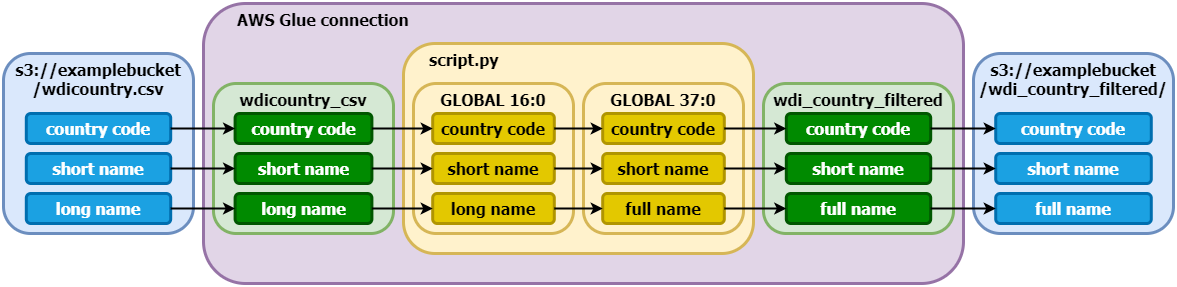
\includegraphics[width=1.0\textwidth]{img/catalog_lineage.png}
\caption{An example of data lineage graph containing Data Catalog tables}
\label{fig:catalogLineage}
\end{figure}

\section{Design of AWS Glue scanner}

The analysis from the previous section creates a strong foundation upon which we can build the design of AWS Glue scanner. We were thinking ahead when creating this design so it covers not only the features implemented in the MVP included in this work, but also the features that were not required in the MVP but need to be implemented in near future to create a full-fledged scanner.
\par
AWS Glue scanner is designed in a standard way consisting of two main components: Connector and Dataflow Generator. The task of the Connector is to connect to AWS Glue, extract all required metadata and transform it into a general model that can be used for data flow analysis. Dataflow Generator uses this model to analyze data flows and create a data lineage graph. 

\subsection{Connection scope}
Each scenario executed in Manta Flow CLI analyzes a single connection to a data technology. The first thing we need to specify is the scope of a connection in AWS Glue. Usually, this scope is defined by connection URL (where available) and credentials. A scenario then analyzes everything it has access to using these connection settings. It makes sense to use this approach in AWS Glue as well. A connection in AWS Glue scanner is defined by credentials and AWS region. This pairing uniquely identifies an AWS Glue service instance (a service instance can be identified by an AWS account ID, which we can obtain from credentials, and by an AWS region). This connection provides access to a set of ETL jobs and Data Catalog which represent the connection's scope of the data flow analysis. The access can be restricted by permissions set in AWS IAM service.

\subsection{AWS Glue Connector design}
AWS Glue Connector takes care of extracting and storing metadata from AWS Glue and resolving the inputs for data flow analysis. The connector is divided into 4 main components, as is common with other scanners:
\begin{enumerate}
    \item \textit{Extractor} which extracts metadata from AWS Glue
    \item \textit{Model} which contains the definition of the general model of the input
    \item \textit{Resolver} which is an implementation of the general model
    \item \textit{Reader} which reads extracted metadata into model used by Dataflow Generator
\end{enumerate}

\subsubsection{Extractor}
The extractor connects to the AWS Glue service instance and extracts all required metadata, saving them on the file system. To extract the metadata, AWS Java v2 SDK is used. The SDK returns data in its own Java objects. We need to extract Data Catalog metadata and ETL job metadata including job scripts. We must not forget that we also need to extract additional libraries and files which are specified in job arguments.
\par
Extracted metadata must be stored in a convenient format and in a well-defined hierarchy on the file system so that it can be correctly loaded into the model used in the data flow analysis. It is common to store metadata in the format in which it was extracted from data technology. In a situation where retrieval of a particular artifact fails (due to insufficient rights or other error), the user can provide it manually. Users can export AWS Glue metadata in multiple formats (using \texttt{aws-cli}, a command line tool for interacting with AWS services), so we chose JSON format for convenience.
\par
The file hierarchy for extracted metadata has to be unambiguous so that the Reader can read it correctly. We designed the file hierarchy shown in Figure~\ref{fig:hierarchy}. Names enclosed in \texttt{< >} represent variable names based on the actual name of the entity described between \texttt{< >} (\texttt{<job1>} would be replaced by the actual name of the first extracted ETL job etc.). The hierarchy intentionally uses \texttt{<region>} and \texttt{<account-id>} top-most directories. While a connection can only extract metadata in a single region, the name of the region is not a part of any metadata, but is required for correct naming of resources, so we store this value in the name of the directory. Account ID can be inferred from Catalog ID stored in table and database metadata, but this value is not present in job metadata and we need it to correctly resolve which Data Catalog is used in job scripts (when no Catalog ID is used when accessing Data Catalog resources, the default one is used), so we stored it in the directory name as well. However, it has another reason. It is possible to use Data Catalog belonging to another AWS account in ETL jobs, so when its metadata is extracted, it is stored in a different directory under that account's ID. Then there are two directories, \texttt{jobs} directory containing ETL job metadata and \texttt{data\_catalog} directory containing Data Catalog metadata. ETL job metadata consist of metadata JSON file and script file, if the job uses additional libraries or files, they would also be stored here. Data Catalog metadata contain JSON files of databases and tables.

\begin{figure}[ht]\centering
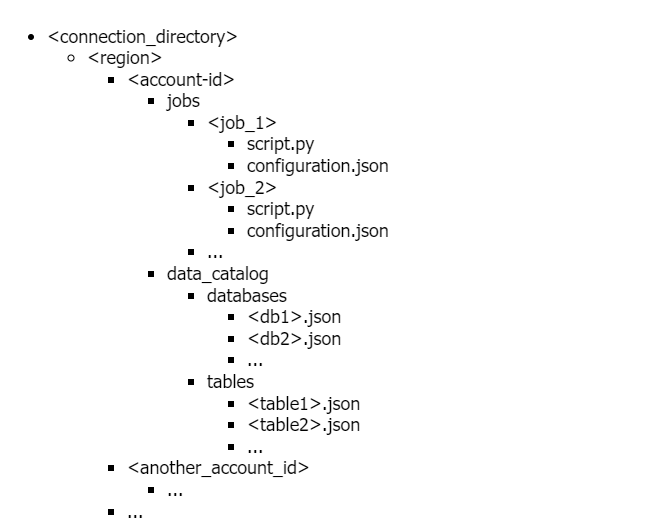
\includegraphics[width=1.0\textwidth]{img/file_hierarchy.png}
\caption{File hierarchy of extracted AWS Glue metadata}
\label{fig:hierarchy}
\end{figure}

\subsubsection{Model, Resolver and Reader}
Model component defines a common data interface of the entities of the general model of AWS Glue input following the principle of loose coupling.
\par
Resolver component contains implementations of Model interfaces. Classes are designed to be immutable so the input for the data flow analysis cannot be accidentally modified.
\par
Reader component takes care of reading the extracted metadata and creating its object representation using the classes defined in the Resolver.

\subsection{AWS Glue Dataflow Generator design}

AWS Glue Dataflow Generator analyzes data flows in the extracted inputs and creates a data lineage graph. Analyzing ETL jobs is fairly simple, all that the Generator needs to do is to call Embedded Code Service. After that it merges the result graph into the AWS Glue graph containing a node representing the job and the work is done. A more interesting problem is the analysis of Data Catalog metadata.
\par
The goal of Data Catalog analysis is to create data flow edges between the nodes representing Data Catalog tables and the nodes representing the actual data sources as well as adding edges when these tables are used in ETL jobs. There are two possibilities how we can achieve that.
\par
The first approach can create a more precise data lineage, but this lineage is only created when Data Catalog is used from AWS Glue (other AWS services can also use Data Catalog, for example AWS Athena can use Data Catalog tables in SQL queries). When ETL jobs are analyzed by Embedded Code Service, the resulting graph shall contain pin nodes representing reads and writes to Data Catalog tables. Then, Dataflow Generator would create the node for this table and map the pin node to the table node. Dataflow generator would also create data source node that the table is mapped to and link it with the table node. In case of Python, table schema could be passed directly to Python analysis using Outsight to provide a more detailed column-level lineage.
\par
The second approach is a more general solution. Firstly, Data Catalog metadata would be stored in a data dictionary so it could be accessed by Dataflow Query Service. Since mapping between the data source and Data Catalog table is visualized as a data flow, it is also possible to create these flows in an extra data flow scenario. Such scenario would create data flows from data sources to Data Catalog tables for all tables present in extracted metadata. Python scanner would use Dataflow Query Service to resolve Data Catalog accesses without the need to create any extra data flows to data sources, because they would already exist. However, since there would be only dataflows from data sources to catalog tables, edges in the other direction (backlinks, when data is written to Data Catalog table) would have to be added in a postprocessing scenario.
\par
The second solution provides more value and the lineage can also be reused for other scanners, that is why we prefer it. However, it implies that several new components need to be developed, namely:
\begin{enumerate}
    \item Data dictionary mapping scenario for mapping Data Catalog metadata into a data dictionary
    \item Data Catalog data flow scenario for creating data flows between Data Catalog tables and their data sources
    \item Specific Dataflow Query Service implementation for AWS Glue Data Catalog
    \item Backlink mapping configuration for adding a missing edge between Data Catalog table and data source when data is written to the table
\end{enumerate}

\section{Implementation of AWS Glue scanner}
In this work we implemented a MVP of AWS Glue scanner. The goal of this MVP was not to create a full-fledged scanner, but to be able to demonstrate the functionality of Embedded Code Service. The implementation can be developed in the future following the presented design. As some of the designed features are implemented in the MVP and some are not, here is a comprehensive list that sums it up:
\begin{itemize}
    \item Implemented features
    \begin{itemize}
        \item Extraction of ETL job metadata and scripts
        \item Data flow analysis of ETL jobs
        \item Creating data lineage graph
        \item Integration with Manta Flow
        \item Configuration in Admin UI
        \item Plugin for analyzing \textit{awsglue} library function calls in Python scanner
        \item Agent for AWS Glue
    \end{itemize}
    \item Unimplemented features
    \begin{itemize}
        \item Extraction of Data Catalog metadata
        \item Extraction of additional files
        \item Data flow analysis of Data Catalog    
    \end{itemize}
\end{itemize}
\par
Let us mention interesting parts from the implementation of some of the features.

\subsection{Extraction}
AWS SDK used for metadata extraction always provides responses to requests deserialized in the form of a Java object. We have stated that we want to store metadata in a serialized JSON format. To avoid implementing serialization logic, we developed a response \textit{interceptor} (\texttt{GlueClientExecutionInterceptor} class) that intercepts a HTTP response before it is deserialized. At this point, the body of the response contains the metadata in the desired JSON format, so we copy it and let the response be deserialized, because it is also convenient to read some of the metadata from the provided response object.
\par
We have also implemented a Manta Flow Agent specialization for AWS Glue extraction. Manta Flow Agent is an application for metadata extraction. In enterprises, it is common to limit access to certain networks for security reasons. Agent was created to allow extracting metadata from systems that are not accessible from the same network as Manta Flow Server.

\subsection{Manta Flow integration}
AWS Glue scanner is fully integrated with Manta Flow. It is released as one of so-called preview scanners which can be used only in preview mode. The scanner can be configured using Admin UI as all other scanners. The configuration includes specification of credentials and filtering expressions for ETL job names which should be included in the analysis.

 

 
\chapter{Evaluation}

In this chapter, we evaluate the outcomes of the implementation presented in the preceding chapters. The primary goal of our work was data flow analysis of embedded code in context of Manta Flow and we need to assess whether our proposed solution achieved its intended objectives.
\par
In this evaluation, we will use an example of an AWS Glue ETL job. This example demonstrates the usage of Python Embedded Code Service for data flow analysis of embedded code in AWS Glue. It makes sense to evaluate both of these components together, because that is how they are intended to be used. We will present and explain the source of the example and then we will show and assess the resulting data lineage with respect to the predefined objectives.
\par
Note that the presented example was created to showcase the implemented functionality and might not be a real representation of an AWS Glue job. However, it does not mean that the data flow makes no sense or that actual scripts would be completely different, but rather that they would be structured differently and contain additional logic for logging etc. The example is also limited by unimplemented features because some function calls that would be used in a production code are not yet supported in Python scanner.

\section{ETL job example}






Mostly description of tests and that it works. If we are lucky we can run it on some Varo scripts and see how it works.

\section{Future work}
What can be done in the future, we can mention that Databricks is being also implemented in ECS.

%%%%%%%%%%%%%%%%%%%%%%%%%%%%%%%%%%%%%%%%%%%%%%%%%%%%%%%%%
\section{Code snippet example}

\begin{figure}[h!]
\begin{lstlisting}[language=Python] 
pass
\end{lstlisting}
\caption{Sample code for representation}
\label{fig:sample-transform-code}
\end{figure}

%%%%%%%%%%%%%%%%%%%%%%%%%%%%%%%%%%%%%%%%%%%%%%%%%%%%%%%%%%%%%%%%%%%%%%%%%%%%%%%%%%%%%%%%%%%%%%%%%%%


\chapter{Conclusion}

Just a conclusion what was done with what results.


%%% Bibliography
%%%% Bibliography (literature used as a source)
%%%
%%% We employ bibTeX to construct the bibliography. It processes
%%% citations in the text (e.g., the \cite{...} macro) and looks up
%%% relevant entries in the bibliography.bib file.
%%%
%%% The \bibliographystyle command selects, which style will be used
%%% for references from the text. The argument in curly brackets is
%%% the name of the corresponding style file (*.bst). Both styles
%%% mentioned in this template are included in LaTeX distributions.

\bibliographystyle{plainnat}    %% Author (year)
% \bibliographystyle{unsrt}     %% [number]

\renewcommand{\bibname}{Bibliography}

%%% Generate the bibliography. Beware that if you cited no works,
%%% the empty list will be omitted completely.

\bibliography{bibliography}

%%% If case you prefer to write the bibliography manually (without bibTeX),
%%% you can use the following. Please follow the ISO 690 standard and
%%% citation conventions of your field of research.

% \begin{thebibliography}{99}
%
% \bibitem{lamport94}
%   {\sc Lamport,} Leslie.
%   \emph{\LaTeX: A Document Preparation System}.
%   2nd edition.
%   Massachusetts: Addison Wesley, 1994.
%   ISBN 0-201-52983-1.
%
% \end{thebibliography}

\printbibliography

%%% Figures used in the thesis (consider if this is needed)
%\listoffigures

%%% Tables used in the thesis (consider if this is needed)
%%% In mathematical theses, it could be better to move the list of tables to the beginning of the thesis.
%\listoftables

%%% Abbreviations used in the thesis, if any, including their explanation
%%% In mathematical theses, it could be better to move the list of abbreviations to the beginning of the thesis.
%\chapwithtoc{List of Abbreviations}

%%% Attachments to the master thesis, if any. Each attachment must be
%%% referred to at least once from the text of the thesis. Attachments
%%% are numbered.
%%%
%%% The printed version should preferably contain attachments, which can be
%%% read (additional tables and charts, supplementary text, examples of
%%% program output, etc.). The electronic version is more suited for attachments
%%% which will likely be used in an electronic form rather than read (program
%%% source code, data files, interactive charts, etc.). Electronic attachments
%%% should be uploaded to SIS and optionally also included in the thesis on a~CD/DVD.
%%% Allowed file formats are specified in provision of the rector no. 72/2017.
\appendix
\chapter{Attachments}

\section{First Attachment}

\openright
\end{document}
